\setchapterpreamble[u]{\margintoc}
\chapter{Command Line Editors}
\labch{clie}

\section{Introduction}

Now that we know how to go about navigating the linux based operating systems, we might want to view and edit files.
This is where command line editors come in.

\begin{definition}
A \textbf{command line editor} is a type of text editor that operates entirely from the command line interface.
They usually do not require a graphical user interface or a mouse.
\footnote{
  This means that CLI editors are the only way to edit files when you are connected to a remote server.
  Since remote servers do not have any graphical server like X11, you cannot use graphical editors like gedit or kate.
}
\end{definition}

\subsection{Types of Editors}

\begin{itemize}

\item \textbf{Graphical Editors:} These are editors that require a graphical user interface.
  Examples include \textit{gedit}
  \footnote{
    Gedit is the default text editor in GNOME desktop environment.
  }
  , \textit{kate}
  \footnote{
    Kate is the default text editor in KDE desktop environment.
  }
  , \textit{vs code}, etc.

\item \textbf{Command Line Editors:} These are editors that operate entirely from the command line interface.

\end{itemize}

We will be only discussing command line editors in this chapter.

\subsection{Why Command Line Editors?}

Command line editors are very powerful and efficient.
They let you edit files without having to leave the terminal.
This is usually faster than opening a graphical editor.
In many cases like sshing
\sidenote{
  SSH stands for Secure Shell.
  It is a cryptographic network protocol for operating network services securely over an unsecured network.
  This will be discussed in detail in a later chapter.
}
into a remote server, command line editors are the only way to edit files.
Another reason for the popularity of command line editors is that they are very lightweight.

\subsection{Mouse Support}
Most command line editors do not have mouse support, and others do not encourage it.
But wont it be difficult to navigate without a mouse?
Not really.
Once you get used to the keyboard shortcuts, you will find that you can navigate way faster than with a mouse.

Mouse editors usually require the user to click on certain buttons,
or to follow multi-click procedures in nested menus to perform certain tasks.

Whereas in keyboard based editors, all the actions that can be performed
are mapped to some keyboard shortcuts.

Modern CLI editors usually also allow the user to totally customize the keyboard shortcuts.

This being said, most modern CLI editors do have mouse support as well if the user is running them in a terminal emulator that supports mouse over a X11 or Wayland display server.
\sidenote{
  X11 and Wayland are display servers that are used to render graphical applications.
  Although not directly covered, these can be explored in details on the
  \href{https://en.wikipedia.org/wiki/Wayland\_(protocol)\#Differences\_between\_Wayland\_and\_X}{internet}.
}

\subsection{Editor war}

Although there are many command line editors available, the most popular ones are \textit{vim} and \textit{emacs}.

\begin{definition}
The editor war is the rivalry between users of the Emacs and vi (now usually Vim, or more recently Neovim) text editors.
The rivalry has become an enduring part of hacker culture and the free software community.
\sidenote{
  More on this including the history and the humor can be found on the
  \href{https://en.wikipedia.org/wiki/Editor\_war}{internet}.
}
\end{definition}

\textbf{Vim}

Vim is a modal editor, meaning that it has different modes for different tasks.
Most editors are modeless, this makes vim a bit difficult to learn.
However, once familiar with it, it is very powerful and efficient.
Vim heavily relies on alphanumeric keys for navigation and editing.
Vim keybindings are so popular that many other editors and even
some browsers
\sidenote{
  \textit{qutebrowser} is a browser that uses vim-like keybindings.
  Firefox and Chromium based browsers also have extensions that provide vim-like keybindings.
  These allow the user to navigate the browser using vim-like keybindings and without ever touching the mouse.
}
have vim-like keybindings.

\textbf{Emacs}

Emacs is a modeless editor, meaning that it does not have different modes for different tasks.
Emacs is also very powerful and efficient.
It uses multi-key combinations for navigation and editing.

\subsection{Differences between Vim and Emacs}
\textbf{Keystroke execution}

Emacs commands are key combinations for which modifier keys are held down while other keys are pressed; a command gets executed once completely typed.

Vim retains each permutation of typed keys (e.g. order matters). This creates a path in the decision tree which unambiguously identifies any command.

\textbf{Memory usage and customizability}

Emacs executes many actions on startup, many of which may execute arbitrary user code. This makes Emacs take longer to start up (even compared to vim) and require more memory. However, it is highly customizable and includes a large number of features, as it is essentially an execution environment for a Lisp program designed for text-editing.

Vi is a smaller and faster program, but with less capacity for customization. vim has evolved from vi to provide significantly more functionality and customization than vi, making it comparable to Emacs.

\textbf{User environment}

Emacs, while also initially designed for use on a console, had X11 GUI support added in Emacs 18, and made the default in version 19. Current Emacs GUIs include full support for proportional spacing and font-size variation. Emacs also supports embedded images and hypertext.

Vi, like emacs, was originally exclusively used inside of a text-mode console, offering no graphical user interface (GUI). Many modern vi derivatives, e.g. MacVim and gVim, include GUIs. However, support for proportionally spaced fonts remains absent. Also lacking is support for different sized fonts in the same document.

\textbf{Function/navigation interface}

Emacs uses metakey chords. Keys or key chords can be defined as prefix keys, which put Emacs into a mode where it waits for additional key presses that constitute a key binding. Key bindings can be mode-specific, further customizing the interaction style. Emacs provides a command line accessed by M-x that can be configured to autocomplete in various ways. Emacs also provides a defalias macro, allowing alternate names for commands.

Vi uses distinct editing modes. Under "insert mode", keys insert characters into the document. Under "normal mode" (also known as "command mode", not to be confused with "command-line mode", which allows the user to enter commands), bare keypresses execute vi commands.

\textbf{Keyboard}

The expansion of one of Emacs' backronyms is Escape, Meta, Alt, Control, Shift, which neatly summarizes most of the modifier keys it uses, only leaving out Super. Emacs was developed on Space-cadet keyboards that had more key modifiers than modern layouts. There are multiple emacs packages, such as spacemacs or ergoemacs that replace these key combinations with ones easier to type, or customization can be done ad hoc by the user.

Vi does not use the Alt key and seldom uses the Ctrl key. vi's keyset is mainly restricted to the alphanumeric keys, and the escape key. This is an enduring relic of its teletype heritage, but has the effect of making most of vi's functionality accessible without frequent awkward finger reaches.

\textbf{Language and script support}

Emacs has full support for all Unicode-compatible writing systems and allows multiple scripts to be freely intermixed.

Vi has rudimentary support for languages other than English. Modern Vim supports Unicode if used with a terminal that supports Unicode.

\subsection{Nano: The peacemaker amidst the editor war}

\textit{Nano} is a simple command line editor that is easy to use.
It does not have the steep learning curve of vim or emacs.
But it is not as powerful as vim or emacs as well.
It is a common choice for beginners who just want to append a few lines to a file or make a few changes.
It is also a non-modal editor like editor which uses modifier chording like emacs.
However, it mostly uses the control key for this purpose and has only simple
keybindings such as \textit{Ctrl+O} to save and \textit{Ctrl+X} to exit.

\section{Vim}

\subsection{History}

The history of Vim is a very long and interesting one.

\begin{table}[h!]
\caption{History of Vim}
\labtab{vimhistory}
\centering
\begin{minipage}[t]{.7\linewidth}
\color{gray}
\rule{\linewidth}{1pt}
\ytl{1967}{QED text editor by Butler Lampson and Peter Deutsch for Berkeley Timesharing System}
\ytl{1967}{Ken Thompson and Dennis Ritchie's QED for MIT CTSS, Multics, and GE-TSS}
\ytl{1969}{Ken Thompson releases ed - The Standard Text Editor}
\ytl{1976}{George Coulouris and Patrick Mullaney release em - The Editor for Mortals}
\ytl{1976}{Bill Joy and Chuck Haley build upon em to make en, which later becomes ex}
\ytl{1977}{Bill Joy adds visual mode to ex}
\ytl{1979}{Bill Joy creates a hardlink `vi` for ex's visual mode}
\ytl{1987}{Tim Thompson develops a vi clone for the Atari ST named STevie (ST editor for VI enthusiasts)}
\ytl{1988}{Bram Moolenaar makes a stevie clone for the Amiga named Vim (Vi IMitation)}
\bigskip
\rule{\linewidth}{1pt}
\end{minipage}
\end{table}

\textbf{Teletypes}

\begin{definition}
A \textbf{teletype} (TTY) or a teleprinter is a device that can send and receive typed messages from a distance.
\end{definition}

\begin{marginfigure}
  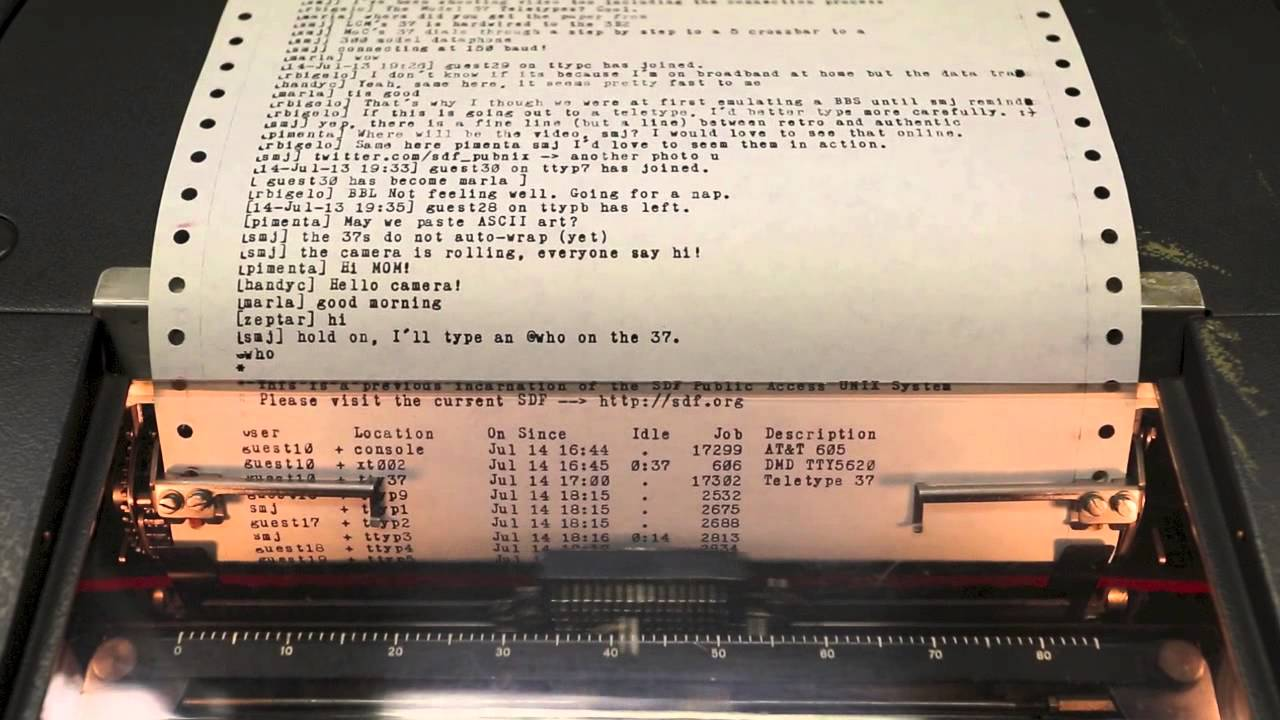
\includegraphics[width=\linewidth]{tty}
  \caption{A Teletype}
	\labfig{tty}
\end{marginfigure}

Very early computers used to use teletypes as the output device.
These were devices that used ink and paper to actually
\textit{print} the output of the computer.
These did not have an \textit{automatic} refresh rate like modern monitors.
Only when the computer sent a signal to the teletype, would the teletype print the output.

Due to these restrictions it was not economical or
practical to print the entire file on the screen.
Thus most editors used to print only one line at a time on the screen
and did not have updating graphics.

\textbf{QED}

\begin{marginfigure}
  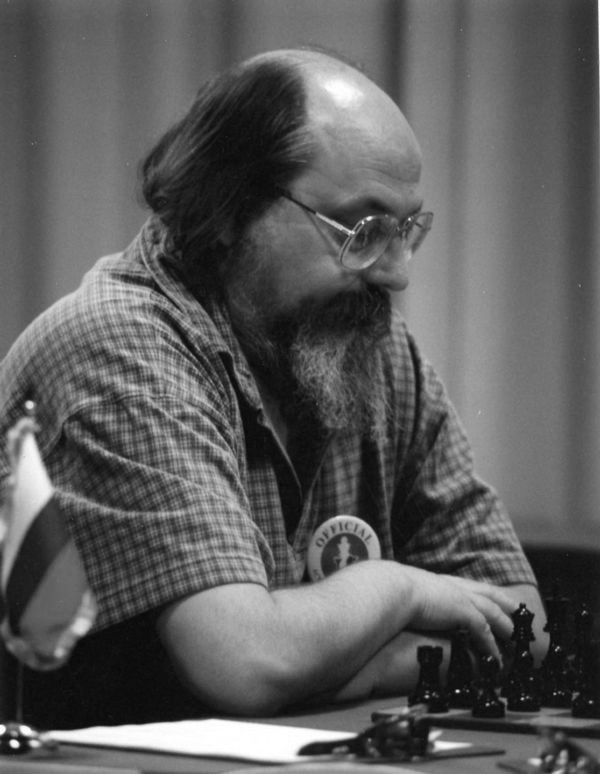
\includegraphics{thompson}
	\caption{Ken Thompson}
	\labfig{thompson}
\end{marginfigure}

QED was a text editor developed by Butler Lampson and Peter Deutsch in 1967 for the Berkeley Timesharing System.
It was a character-oriented editor that was used to create and edit text files.
It used to print or edit only one character at a time on the screen.
This is because the computers at that time used to use
a teletype machine as the output device, and not a monitor.

Ken Thompson used this QED at Berkeley before he came to Bell Labs, and among the first things he did on arriving was to write a new version for the MIT CTSS system.
Written in IBM 7090 assembly language, it differed from the Berkeley version most notably in introducing regular expressions
\sidenote{
  Regular expressions are a sequence of characters that define a search pattern.
  Usually this pattern is used by string searching algorithms for "find" or "find and replace" operations on strings.
  This will be discussed in detail in a later chapter.
}
for specifying strings to seek within the document being edited, and to specify a substring for which a substitution should be made.
Until that time, text editors could search for a literal string, and substitute for one, but not specify more general strings.

Ken not only introduced a new idea, he found an inventive implementation: on-the-fly compiling. Ken's QED compiled machine code for each regular expression that created a NDFA (non-deterministic finite automaton) to do the search. He published this in C. ACM 11 \#6, and also received a patent for the technique: US Patent \#3568156.

\begin{marginfigure}
  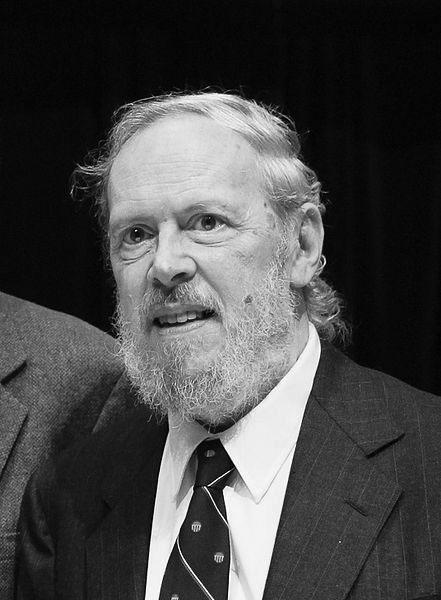
\includegraphics{ritchie}
	\caption{Dennis Ritchie}
	\labfig{ritchie}
\end{marginfigure}

While the Berkeley QED was character-oriented, the CTSS version was line-oriented. Ken's CTSS qed adopted from the Berkeley one the notion of multiple buffers to edit several files simultaneously and to move and copy text among them, and also the idea of executing a given buffer as editor commands, thus providing programmability.

When developing the MULTICS project, Ken Thompson wrote yet another version of QED for that system, now in BCPL
\sidenote{
BCPL ("Basic Combined Programming Language") is a procedural, imperative, and structured programming language. Originally intended for writing compilers for other languages, BCPL is no longer in common use.
}
and now created trees for regular expressions instead of compiling to machine language.

In 1967 when Dennis Ritchie joined the project, Bell Labs had slowly started to move away from Multics. While he was developing the initial stages of Unix, he rewrote QED yet again, this time for the GE-TSS system in Assembly language.
This was well documented, and was originally intented to be published as a paper.
\sidenote{
  At that time, systems did not have a standardized CPU architecture or a generalized low level compiler.
  Due to this, applications were not portable across systems.
  Each machine needed its own version of the application to be written from the scratch, mostly in assembly language.
}

\marginnote{
  The reference manual for GE-TSS QED can still be found on
  \href{https://www.bell-labs.com/usr/dmr/www/qedman.pdf}{Dennis Ritchie's website}
  Much of this information is taken from his
  \href{https://www.bell-labs.com/usr/dmr/www/qed.html}{blog}.
}

\textbf{ED}

After their experience with multiple implementations of QED,
Ken Thompson wrote \textbf{ed} in 1969.

This was now written in the newly developed B language, a predecessor to C.
This implementation was much simpler than QED, and was line oriented.
It stripped out much of regular expression support, and only had the support
for \texttt{*}.
It also got rid of multiple buffers and executing contents of buffer.

Slowly, with time, Dennis Ritchie created the C language, which is widely in use
even today.

Ken Thompson re-wrote \textbf{ed} in C, and added back some of the
complex features of QED, like back references in regular expressions.

Ed ended up being the \textbf{Standard Text Editor} for Unix systems.

\begin{remark}
Since all of Bell-Labs and AT\&T's software was proprietary, the source code for ed was not available to the public.
Thus, the \textit{ed} editor accessible today in \textbf{GNU/Linux},
is another implementation of the original \textit{ed} editor
by the GNU project.
\end{remark}

However, \textbf{ed} was not very user friendly and it was very terse.
Although this was originally intented, since it would be
very slow to print a lot of diagnostic messages on a teletype,
slowly, as people moved to faster computers and monitors,
they wanted a more user friendly editor.

\textbf{VDU Terminals}

\begin{definition}
  A terminal that uses video display technology like
  cathode rat tubes (CRT) or liquid crystal displays (LCD)
  to display the terminal output is called a \textbf{VDU terminal}.
  (Video Display Unit)
\end{definition}

\begin{marginfigure}
  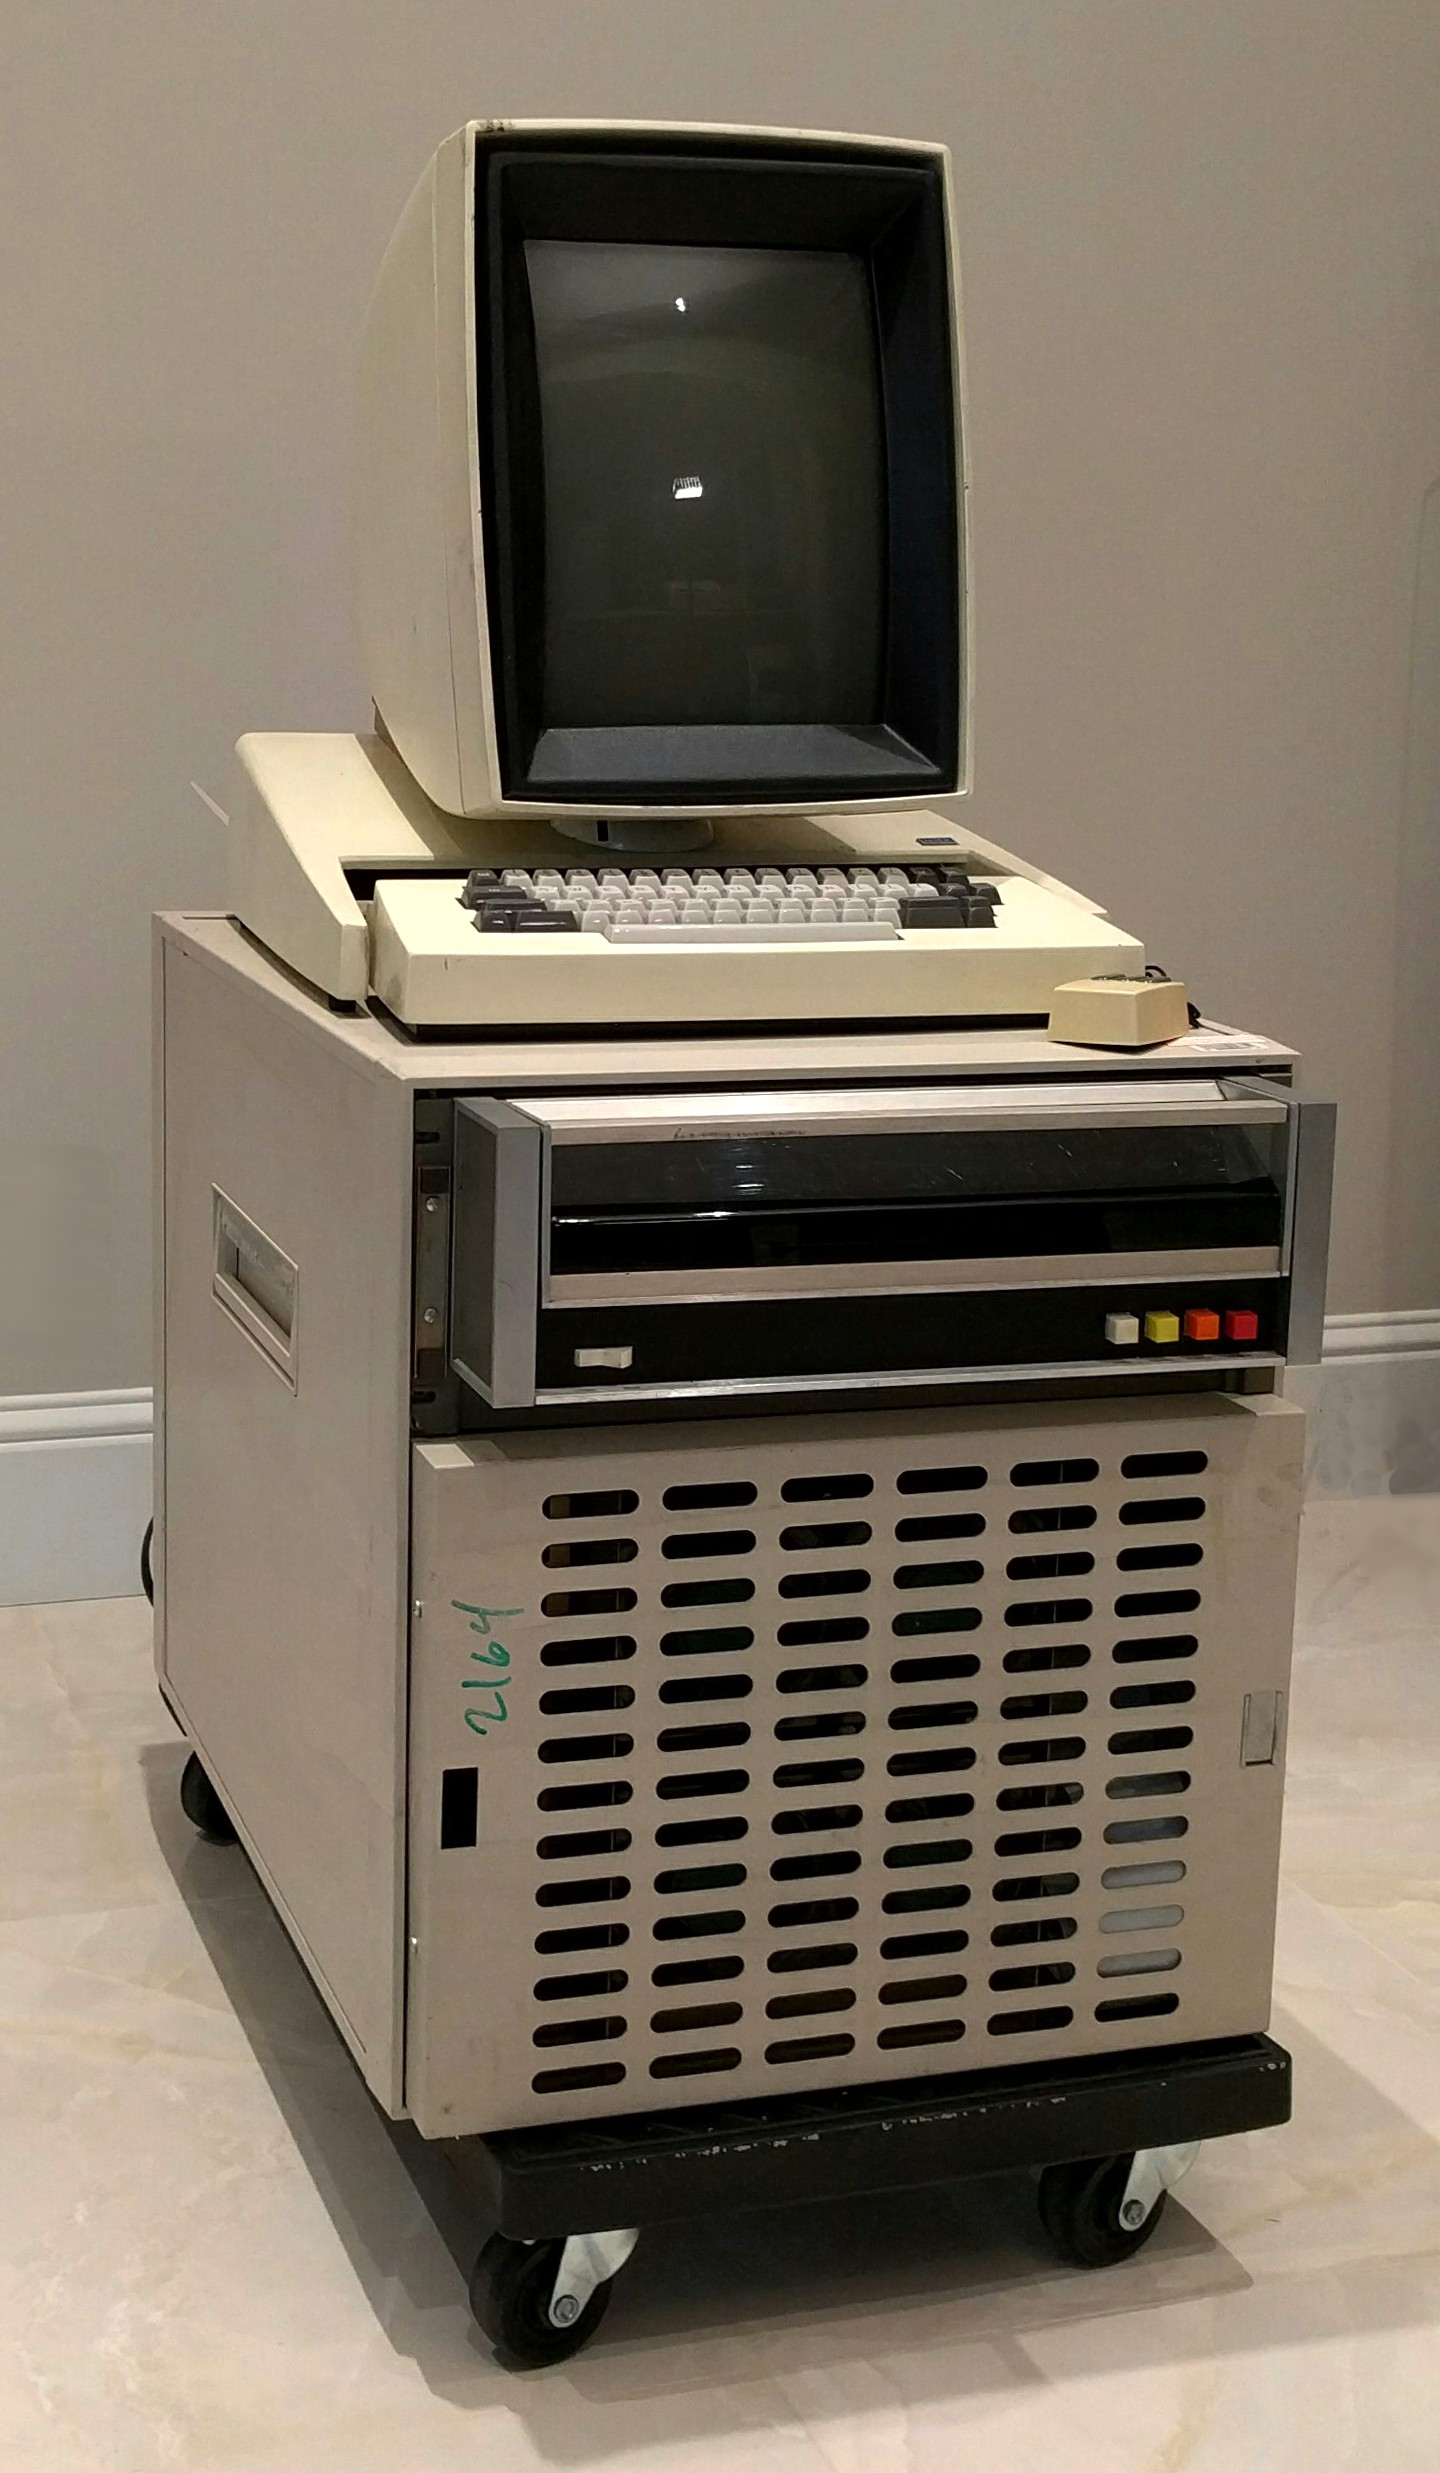
\includegraphics{alto}
  \caption{Xerox Alto, one of the first VDU terminals with a GUI, released in 1973}
	\labfig{alto}
\end{marginfigure}

These terminals were able to show video output, instead of
just printing the output on paper.
Although initially these were very expensive, and were not
a household item, they were present in the research parks
like Xerox PARC.

\textbf{EM}

\href{https://en.wikipedia.org/wiki/George\_Coulouris\_(computer\_scientist)}{George Coulouris}
(not the actor)
was one of the people who had access to these terminals
in his work at the Queen Mary College in London.

The drawbacks of \textbf{ed} were very apparent to him
when using on these machines.

He found that the UNIX's \textbf{raw} mode, which was
at that time totally unused,
could be used to give some of the convenience
and immediacy of feedback for text editing.

He claimed that although the \textbf{ed} editor was
groundbreaking in its time, it was not very user friendly.
He termed it as not being an editor for mortals.

He thus wrote \textbf{em} in 1976, which was an \textbf{Editor for Mortals}.
\sidenote{
  George named em as Editor for Mortals because
  Ken Thompson visited his lab at QMC while he
  was developing it and said something like:
  "yeah, I've seen editors like that,
  but I don't feel a need for them,
  I don't want to see the state of
  the file when I'm editing".
  This made George think that Ken was
  not a mortal, and thus he named it
  Editor for Mortals.
}


\begin{marginfigure}
  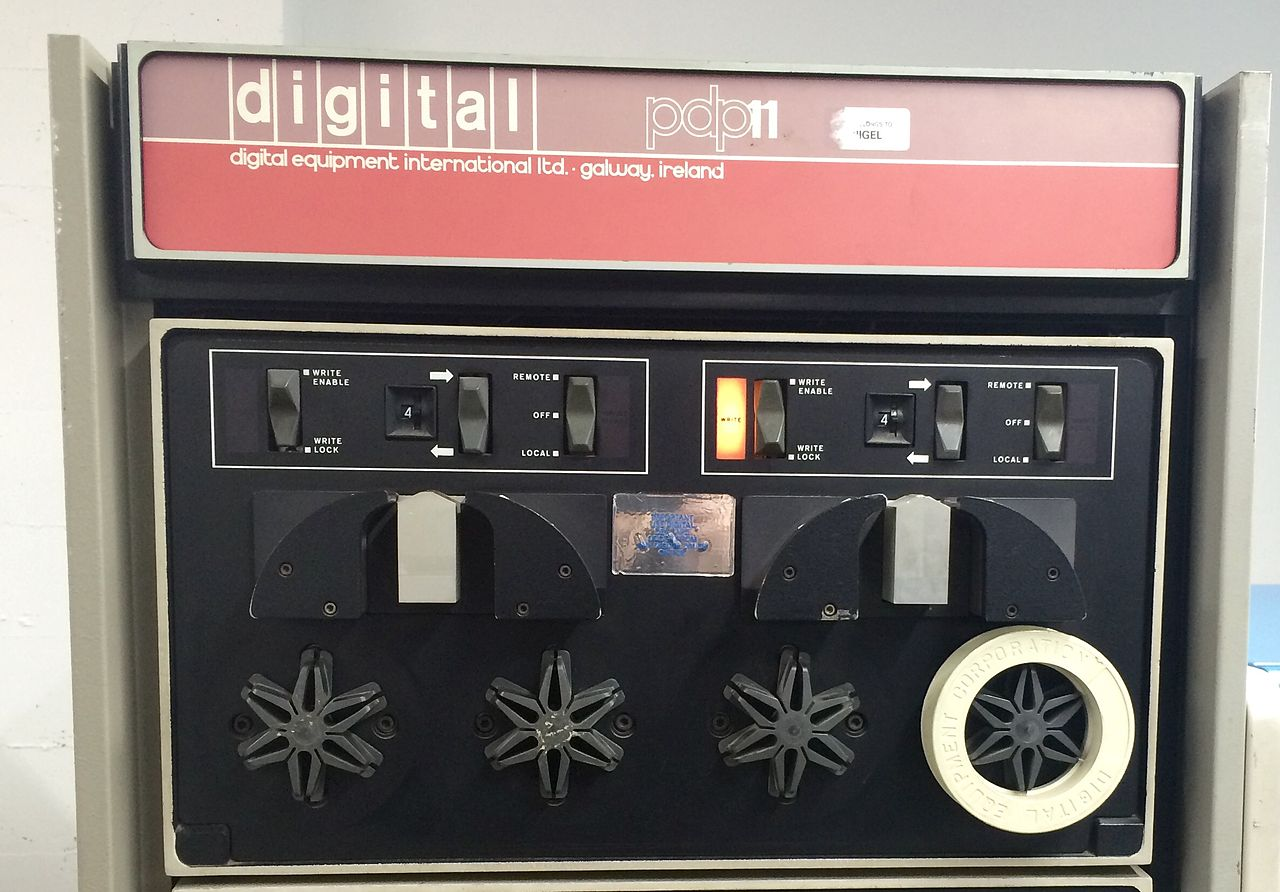
\includegraphics{dectape-pdp11}
  \caption{A first generation Dectape
  (bottom right corner, white round tape)
  being used with a PDP-11 computer}
	\labfig{dectape-pdp11}
\end{marginfigure}

Although em added a lot of features to ed, it was still
a line editor, that is, you could only see one line at a time.
The difference from ed was that it allowed visual editing,
meaning you can see the state of the line as you are editing it.

Whereas most of the development of Multics and Unix
was done in the United States, the development of \textbf{em}
was done in the United Kingdom, in the Queen Mary College,
which was the first college in the UK to have UNIX.

\textbf{EN}

In the summer of 1976, George Coulouris was a visiting professor
at the University of California, Berkeley.
With him, he had brought a copy of his \textbf{em} editor
on a Dectape
\sidenote{
  A Dectape is a magnetic tape storage device that was used in the 1970s.
  It was used to store data and programs.
}
and had installed it there on their departmental computers
which were still using teletype terminals.
Although em was designed for VDU terminals, it was still
able to run (albeit slowly) on the teletype terminals
by printing the current line every time.

\begin{marginfigure}
  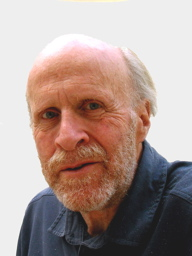
\includegraphics{georgeQMC}
  \caption{George Coulouris}
  \labfig{georgeQMC}
\end{marginfigure}

There he met Bill Joy, who was a PhD student at Berkeley.
On showing him the editor, Bill Joy was very impressed
and wanted to use it on the PDP-11 computers at Berkeley.
The system support team at Berkley were using PDP-11 which
used VDU Terminals, an environment where em would really shine.

He explained that 'em' was an extension of 'ed'
that gave key-stroke level interaction for editing
within a single line, displaying the up-to-date line
on the screen (a sort of single-line screen editor).
This was achieved by setting the terminal mode to 'raw'
so that single characters could be read as they were typed
- an eccentric thing for a program to do in 1976.

Although the system support team at Berkeley were
impressed by this editor, they knew that if this
was made available to the general public, it would
take up too much resources by going to the raw mode
on every keypress.
But Bill and the team took a copy of the source code
just to see if they might use it.

George then took a vacation for a few weeks,
but when he returned, he found that Bill had
taken his ex as a starting point and had
added a lot of features to it. He called it
\textbf{en} initially, which later became \textbf{ex}.

\textbf{EX}

\begin{marginfigure}
  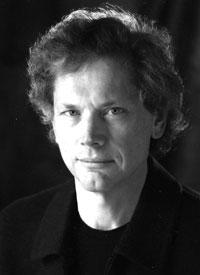
\includegraphics{billjoy}
  \caption{Bill Joy}
  \labfig{billjoy}
\end{marginfigure}


Bill Joy took inspiration from several other ed clones as well,
and their own tweaks to ed,
although the primary inspiration was \textbf{em}.
Bill and Chuck Haley built upon em to make en, which later became ex.

This editor had a lot of improvements over em,
such as adding the ability to add abbreviations
(using the \texttt{ab} command),
and adding keybindings (maps).

It also added the ability to mark some line
using the \texttt{k} key followed by any letter,
and then jump to that line from any arbitrary line
using the \texttt{'} key followed by the letter.

Slowly, with time, the modern systems were able able
to handle the raw mode, and real time editing more and more.
This led to the natural progression, What if we could
see the entire file at once, and not just one line at a time?

\textbf{VI}

Bill added the \textbf{visual mode} to ex in 1977.
\sidenote{
  This visual mode is not the same as the visual mode in vim.
}
This was not a separate editor, but rather just another mode
of the \textbf{ex} editor.
You could open ex in visual mode using the \texttt{-v} flag to
ex.

\begin{lstlisting}[language=bash]
$ ex -v filename
\end{lstlisting}

This visual mode was the first time a text editor
was \textbf{modal}.
This means that the editor had different modes for different tasks.
When you want to edit text, you would go to the insert mode,
and type the text.
When you want to navigate, you would go to the normal mode,
and use the navigation keys and other motions defined in vi.

Slowly, as the visual mode became more and more popular,
Bill added a hardlink to ex called \textbf{vi}.
\sidenote{
  This means that it did not take up additional space on the disk,
  but was just another entry in the directory entry that pointed
  to the same inode which stored the ex binary path.
  Upon execution, \textbf{ex} would detect if it was
  called as \textbf{vi} and would start in visual mode by default.
  We have covered hardlinks in \refch{basic}.
}

The modal version of vi was also inspired from another
editor called \textbf{bravo}, which was developed at Xerox PARC.
\sidenote{
  Xerox PARC has always been ahead of its time.
  The first graphical user interface was developed at Xerox PARC.
  The bravo editor used bitmapped graphics to display the text,
  and had extensive mouse support.
  The overdependence on the mouse in such an early time
  was one of the reasons that the bravo editor was not
  as popular as vi.
}

If you use vi/vim, you may notice that the key to
exit the insert mode is \texttt{Esc}.
This may seem inconveniently placed at the top left corner,
but this was because the original vi was developed on a
ADM-3A terminal, which had the \texttt{Esc} key to the left
of the \textbf{Q} key, where modern keyboards have the \texttt{Tab} key.
\sidenote{
  Since the placement of the Escape key is inconvenient
  in modern keyboard layouts, many people remap the
  Escape key to the \texttt{Caps Lock} key either in vim
  or in the operating system itself.
}

Also, the choice of h,j,k,l for navigation was because
the ADM-3A terminal did not have arrow keys,
rather, it had h,j,k,l keys for navigation.

This can be seen in \reffig{adm3a}.

\begin{figure}[h!]
  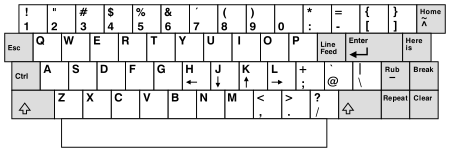
\includegraphics{adm3a}
  \caption{The Keyboard layout of the ADM-3A terminal}
  \labfig{adm3a}
\end{figure}


Bill Joy was also one of the people working on the
\textbf{Berkeley Software Distribution (BSD) of Unix}.
Thus he bundled vi with the first BSD distribution of UNIX
released in 1978.
The pre-installed nature of vi in the BSD Distribution
made it very popular.

However, since both the source code of ed was restricted by
Bell Labs - AT\&T, and the source code of vi was restricted
by the University of California, Berkeley,
they could not be modified by the users or distributed freely.

This gave birth to a lot of clones of vi.

\textbf{Vi Clones}

The vi clones were written because the source code for the original version was not freely available until recently. This made it impossible to extend the functionality of vi. It also precluded porting vi to other operating systems, including Linux.

\begin{marginfigure}
  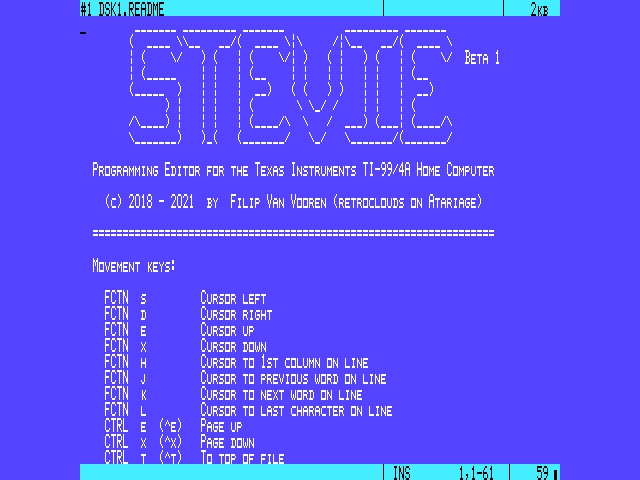
\includegraphics{stevie}
  \caption{Stevie Editor}
  \labfig{stevie}
\end{marginfigure}

\begin{itemize}
  \item \textbf{calvin}: a freeware "partial clone of vi" for use on MS-DOS.
 It has the advantages of small size (the .exe file is only 46.1KB!) and fast execution but the disadvantage that it lacks many of the ex commands, such as search and replace.
  \item \textbf{lemmy}: a shareware version of vi implemented for the Microsoft Windows platforms which combines the interface of vi with the look and feel of a Windows application.
  \item \textbf{nvi}: It is a re-implementation of the classic Berkeley vi editor, derived from the original 4.4BSD version of vi.
    It is the "official" Berkeley clone of vi, and it is included in FreeBSD and the other BSD variants.
  \item \textbf{stevie}: `ST Editor for VI Enthusiasts` was developed by Tim Thompson for the Atari ST.
    It is a clone of vi that runs on the Atari ST.
    Tim Thompson wrote the code from scratch (not based on vi) and posted its
    source code as a free software to
    \href{https://groups.google.com/g/comp.sys.atari.st}{comp.sys.atari.st}
    on June 1987. Later it was ported to UNIX, OS/2, and Amiga.
    Because of this independence from vi and ed's closed source license,
    most vi clones would base their work off of stevie to keep it free
    and open source.
  \item \textbf{elvis}:
    Elvis creator, Steve Kirkendall, started thinking of writing his own editor after Stevie crashed on him, causing him to lose hours of work and damaging his confidence in the editor.
Stevie stored the edit buffer in RAM, which Kirkendall believed to be impractical on the MINIX operating system. One of Kirkendall's main motivation for writing his own vi clone was that his new editor stored the edit buffer in a file instead of storing it in RAM. Therefore, even if his editor crashed, the edited text could still be retrieved from that external file.
Elvis was one of the first vi clones to offer support for GUI and syntax highlighting.
\end{itemize}

The clones add numerous new features which make them significantly easier to use than the original vi, especially for neophytes.
A particularly useful feature in many of them is the ability to edit files in multiple windows.
This facilitates working on more than one file at the same time, including cutting and pasting text among them.

Many of the clones also offer GUI versions of vi that operate under the X Windows system and can take advantage of bit-mapped (high resolution) displays and the mouse.

\textbf{Vim}

\begin{marginfigure}
  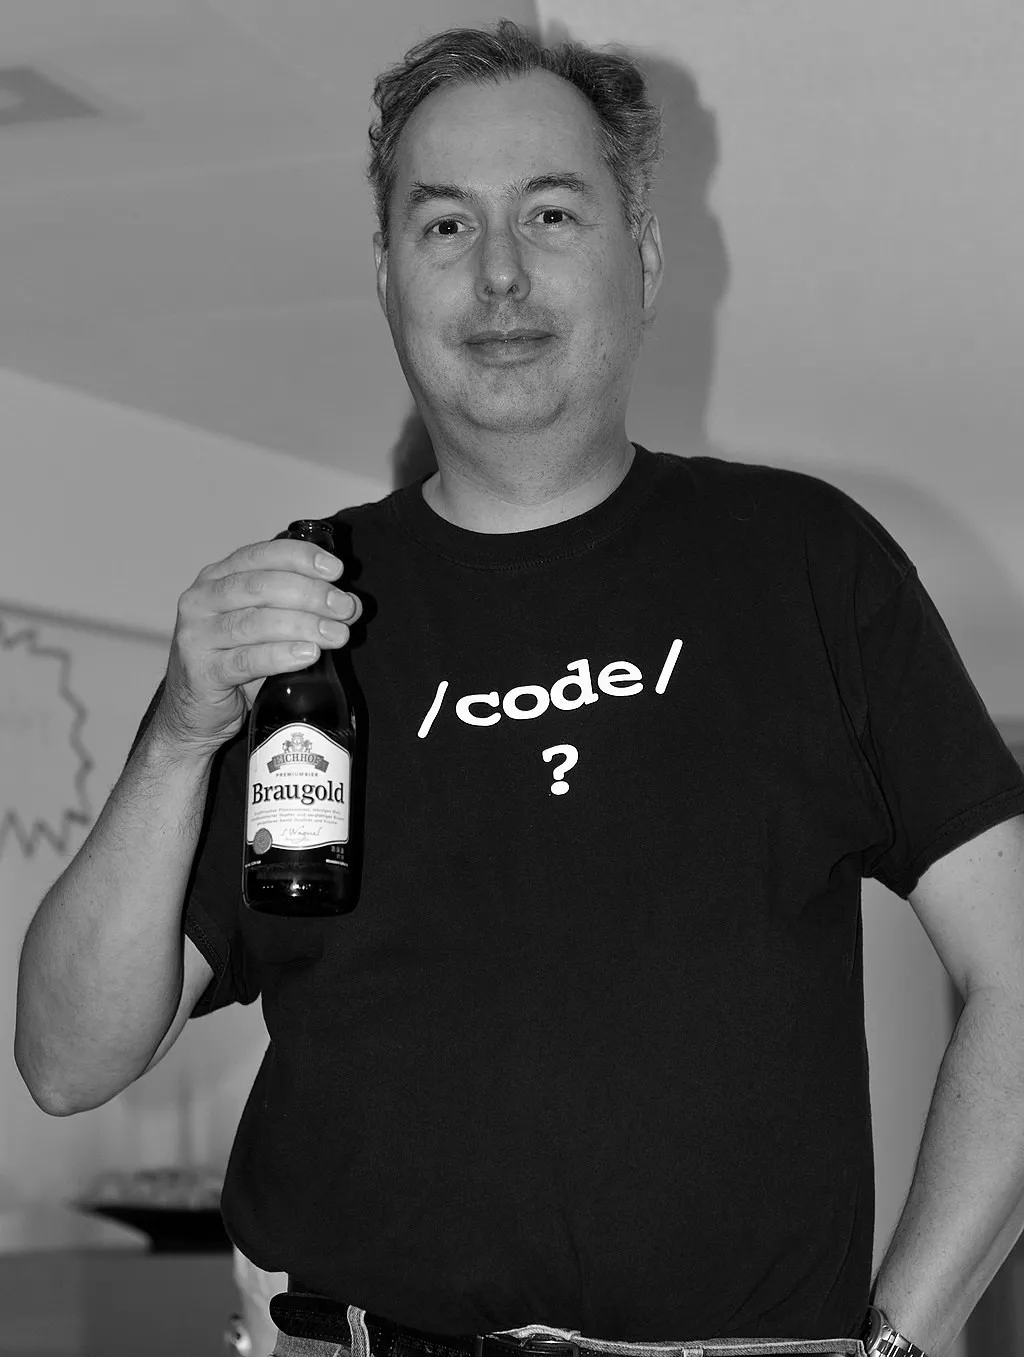
\includegraphics{bram}
  \caption{Bram Moolenaar}
  \labfig{bram}
\end{marginfigure}

Bram Moolenaar, a Dutch programmer, was impressed by
STeVIe, a vi clone for the Atari ST.
But he was working with the Commodore Amiga at that time,
and there was no vi clone for the Amiga.
So Bram began working on the stevie clone
for the AmigaOS in 1988.

\begin{figure}[h!]
  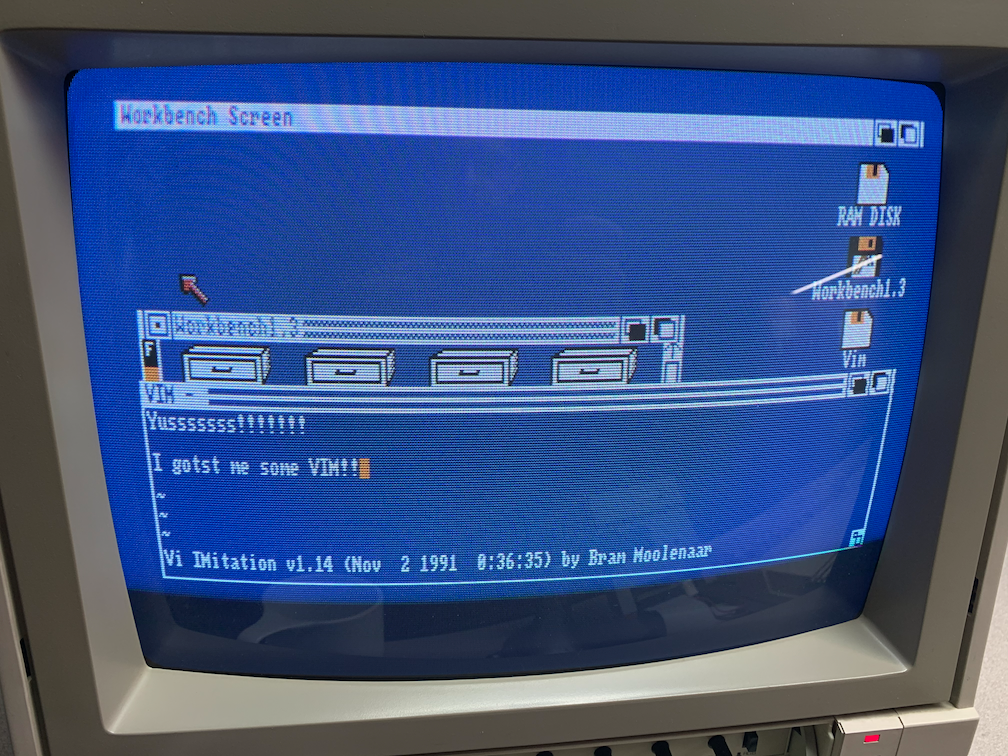
\includegraphics[width=0.8\linewidth]{vim-amiga}
  \caption{The inital version of Vim, when it was called Vi IMitation}
  \labfig{vim-amiga}
\end{figure}

He released the first public release (v 1.14) in 1991
as visible in \reffig{vim-amiga}.

Since Vim was based off of Stevie, and not ed or vi
so it could be freely distributed.
It was licensed under a charityware license,
named as Vim License.
The license stated that if you liked the software,
you should consider making a donation to a charity
of your choice.

Moolenaar was an advocate of a NGO based in Kibaale, Uganda,
which he founded to support children whose parents have died of AIDS.
In 1994, he volunteered as a water and sanitation engineer for the
Kibaale Children's Centre and made several return trips
over the following twenty-five years.

Later Vim was re-branded as `Vi IMproved`
as seen in \reffig{vim}.

\begin{marginfigure}
  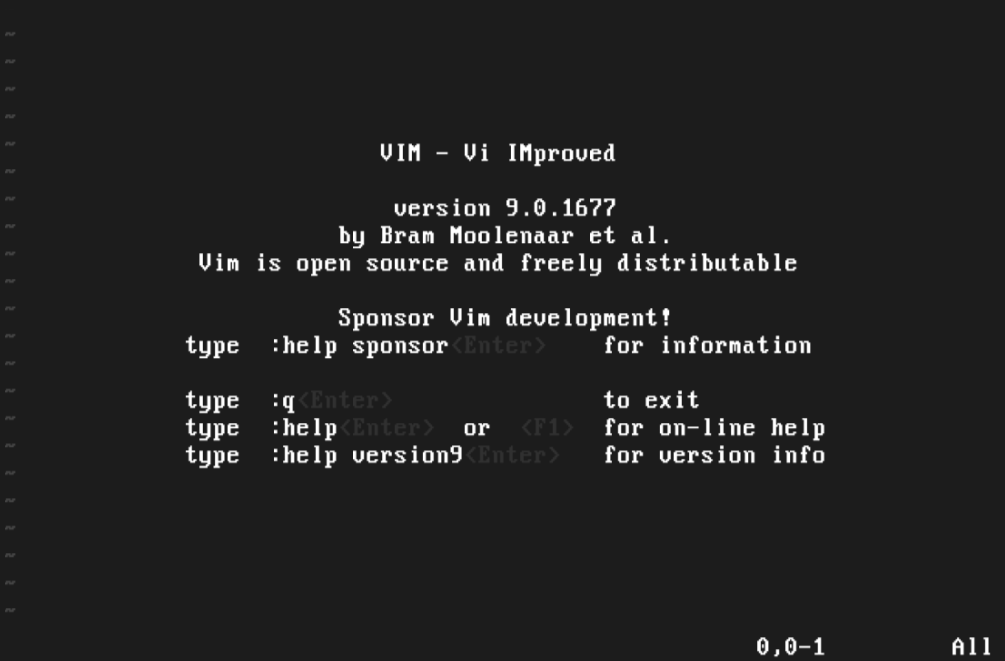
\includegraphics{vim}
  \caption{Vim 9.0 Start screen}
  \labfig{vim}
\end{marginfigure}

Vim has been in development for over 30 years now,
and is still actively maintained.
It has added a lot of features over the years,
such as syntax highlighting, plugins,
completion, PCRE support, mouse support, etc.

\textbf{neovim}

Recently there have been efforts
to modernize the vim codebase.
Since it is more than 30 years old,
it has a lot of legacy code.
The scripting language of vim is
also not a standard programming language,
but rather a custom language called vimscript.

To counter this, a new project called \textbf{neovim}
has been started.
It uses \textbf{lua} as the scripting language,
and has a lot of modern features like
out of the box support for LSP,
\sidenote{
  LSP stands for Language Server Protocol.
  It is a protocol that allows the editor to communicate
  with a language server to provide features like
  autocompletion, go to definition, etc.
  This makes vim more like an IDE.
}
better mouse integration, etc.

In this course, we will be learning only
about basic vi commands and we will be
using vim as the editor.

\begin{figure}[h!]
  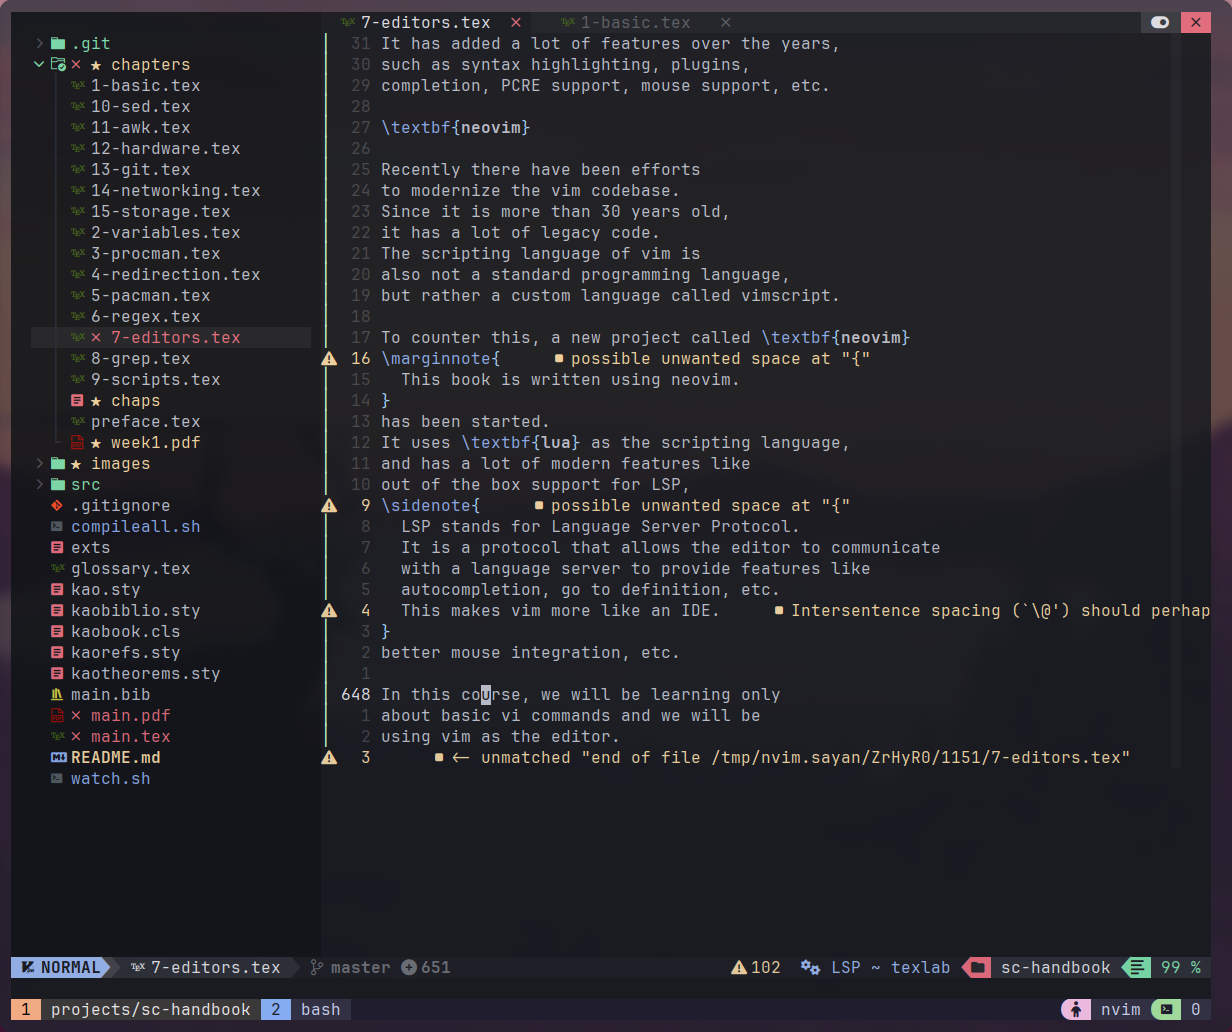
\includegraphics{nvim}
  \caption{Neo Vim Window editing this book}
  \labfig{nvim}
\end{figure}

\marginnote{
  This book is written using neovim.
}

\vfill
\pagebreak

\subsection{Ed Commands}

Before we move on to Vi Commands,
let us first learn about the basic ed commands.
These will also be useful in vim, since the
ex mode of vim is based on ed/ex where we can
directly use ed commands on our file in the buffer.

\begin{table}[h!]
  \caption{Ed Commands}
  \labtab{edcommands}
  \begin{tabular}{l l}
    \toprule
    Description & Commands \\
    \midrule
    Show the \textbf{P}rompt & \texttt{P} \\
    Command Format & \texttt{[addr[,addr]]cmd[params]} \\
    Commands for location & \texttt{1} \texttt{.} \texttt{\$} \texttt{\%} \texttt{+} \texttt{-} \texttt{,} \texttt{;} \texttt{/RE/} \\
    Commands for editing & \texttt{f} \texttt{p} \texttt{a} \texttt{c} \texttt{d} \texttt{i} \texttt{j} \texttt{s} \texttt{m} \texttt{u} \\
    Execute a shell \textit{command} & \texttt{!command} \\
    \textbf{e}dit a file & \texttt{e filename} \\
    \textbf{r}ead file contents into buffer & \texttt{r filename} \\
    \textbf{r}ead \textit{command} output into buffer & \texttt{r !command} \\
    \textbf{w}rite buffer to filename & \texttt{w filename} \\
    \textbf{q}uit & \texttt{q} \\
    \bottomrule
  \end{tabular}
\end{table}

\textbf{Commands for location}

\begin{table}[h!]
  \caption{Commands for location}
  \labtab{ed-location}
\begin{tabular}{ c l }
\toprule
Commands & Description \\
\midrule
a number like \texttt{2} & refers to second line of file \\
\texttt{.} & refers to current line \\
\texttt{\$} & refers to last line \\
\texttt{\%} & refers to all the lines \\
\texttt{+} & line after the cursor (current line) \\
\texttt{-} & line before the cursor (current line) \\
\texttt{,} & refers to buffer holding the file or last line in buffer \\
\texttt{;} & refers to current position to end of the file \\
\texttt{/RE/} & refers line matched by pattern specified by 'RE' \\
\bottomrule
\end{tabular}
\end{table}


\textbf{Commands for Editing}

\begin{table}[h!]
  \caption{Commands for Editing}
  \labtab{ed-editing}
  \begin{tabular}{ c l }
    \toprule
    Commands & Description \\
    \midrule
    \texttt{f} & show name of \textbf{f}ile being edited \\
    \texttt{p} & \textbf{p}rint the current line \\
    \texttt{a} & \textbf{a}ppend at the current line \\
    \texttt{c} & \textbf{c}hange the current line \\
    \texttt{d} & \textbf{d}elete the current line \\
    \texttt{i} & \textbf{i}nsert line at the current position \\
    \texttt{j} & \textbf{j}oin lines \\
    \texttt{s} & \textbf{s}earch for regex pattern \\
    \texttt{m} & \textbf{m}ove current line to position \\
    \texttt{u} & \textbf{u}ndo latest change \\
    \bottomrule
  \end{tabular}
\end{table}

Let us try out some of these commands in the ed editor.

Lets start with creating a file, which we will then open
in the ed editor.

\begin{lstlisting}[language=bash]
$ echo "line-1 hello world
line-2 welcome to line editor
line-3 ed is perhaps the oldest editor out there
line-4 end of file" > test.txt
\end{lstlisting}

This creates a file in the current working directory
with the name \texttt{test.txt} and the contents as
given above.

We invoke ed by using the executable \texttt{ed}
and providing the filename as an argument.

\begin{lstlisting}[language=bash]
$ ed test.txt
117
\end{lstlisting}

As soon as we run it, you will see a number,
which is the number of characters in the file.
The terminal may seem hung, since there is no
prompt, of either the bash shell, or of the ed editor.
This is because ed is a line editor, and it does not
print the contents of the file on the screen.

Off the bat, we can observe the terseness of the ed editor
since it does not even print a prompt.
To turn it on, we can use the \texttt{P} command.
The default prompt is \texttt{*}.

\begin{lstlisting}[language=bash]
ed test.txt
117
P
*
\end{lstlisting}

Now we can see the prompt \texttt{*} is always present,
whenever the ed editor expects a command from the user.

Lets go to the first line of the file using the \texttt{1} command.
We can also go to the last line of the file using the \texttt{\$} command.

\begin{lstlisting}[language=bash]
*1
line-1 hello world
*$
line-4 end of file
*
\end{lstlisting}

To print out all the lines of the file,
we can use the \texttt{,} or \texttt{\%} with \texttt{p} command.

\begin{lstlisting}[language=bash]
*,p
line-1 hello world
line-2 welcome to line editor
line-3 ed is perhaps the oldest editor out there
line-4 end of file
\end{lstlisting}

\begin{lstlisting}[language=bash]
*%p
line-1 hello world
line-2 welcome to line editor
line-3 ed is perhaps the oldest editor out there
line-4 end of file
\end{lstlisting}

However, if we use the \texttt{,} command without
the \texttt{p} command, it will not print all the lines.
Rather, it will just move the cursor to the last line
and print the last line.

\begin{lstlisting}[language=bash]
*,
line-4 end of file
\end{lstlisting}

We can also print any arbitrary line range
using the line numbers separated by a comma
and followed by the \texttt{p} command.

\begin{lstlisting}[language=bash]
*2,3p
line-2 welcome to line editor
line-3 ed is perhaps the oldest editor out there
\end{lstlisting}

One of the pioneering features of ed was the ability
to search for a pattern in the file. Let us quickly
explain the syntax of the search command.
\sidenote{
  The details of regular expressions will be covered in a later chapter.
}

\begin{lstlisting}[language=bash]
*/hello/
line-1 hello world
\end{lstlisting}

We may or may not include the \texttt{p} command
after the last \texttt{/{}} in the search command.

We can advance to the next line using the \texttt{+} command.

\begin{lstlisting}[language=bash]
*p
line-1 hello world
*+
line-2 welcome to line editor
\end{lstlisting}

And go to the previous line using the \texttt{-} command.


\begin{lstlisting}[language=bash]
*p
line-2 welcome to line editor
*-
line-1 hello world
\end{lstlisting}

We can also print all the lines from the current line
to the end of the file using the \texttt{;p} command.

\begin{lstlisting}[language=bash]
*.
line-2 welcome to line editor
*;p
line-2 welcome to line editor
line-3 ed is perhaps the oldest editor out there
line-4 end of file
\end{lstlisting}

We can also run arbitrary shell commands using the \texttt{!} command.

\begin{lstlisting}[language=bash]
*! date
Mon Jun 10 11:36:34 PM IST 2024
!
\end{lstlisting}

The output of the command is shown to the screen,
however, it is not saved in the buffer.

To read the output of a command into the buffer,
we can use the \texttt{r} command.

\begin{lstlisting}[language=bash]
*r !date
32
*%p
line-1 hello world
line-2 welcome to line editor
line-3 ed is perhaps the oldest editor out there
line-4 end of file
Mon Jun 10 11:37:42 PM IST 2024
\end{lstlisting}

The output after running the \texttt{r !date} command
is the number of characters read into the buffer.
We can then print the entire buffer using the \texttt{\%p} command.

The read data is appended to the end of the file.

We can write the buffer
\sidenote{
  Remember that the buffer is the in-memory copy of the file
  and any changes made to the buffer are not saved to the file
  until we write the buffer to the file.
}
to the disk using the \texttt{w} command.

\begin{lstlisting}[language=bash]
*w
149
\end{lstlisting}

The output of the \texttt{w} command is the number of characters written to the file.

To exit ed, we can use the \texttt{q} command.

\begin{lstlisting}[language=bash]
*q
\end{lstlisting}

To delete a line, we can use the \texttt{d} command.
Lets say we do not want the date output in the file.
We can re-open the file in ed and remove the last line.

\begin{lstlisting}[language=bash]
$ ed test.txt
149
P
*$
Mon Jun 10 11:38:49 PM IST 2024
*d
*%p
line-1 hello world
line-2 welcome to line editor
line-3 ed is perhaps the oldest editor out there
line-4 end of file
*wq
117
\end{lstlisting}

We can add lines to the file using the \texttt{a} command.
This appends the line after the current line.
On entering this mode, the editor will keep on taking
input for as many lines as we want to add.
To end the input, we can use the \texttt{.} command on a new line.

\begin{lstlisting}[language=bash]
$ ed test.txt
117
P
*3
line-3 ed is perhaps the oldest editor out there
*a
perhaps not, since we know it was inspired from QED
which was made multiple times by thompson and ritchie
before ed was made.
.
*%p
line-1 hello world
line-2 welcome to line editor
line-3 ed is perhaps the oldest editor out there
perhaps not, since we know it was inspired from QED
which was made multiple times by thompson and ritchie
before ed was made.
line-4 end of file
*
\end{lstlisting}

We can also utilize the regular expression support
in ed to perform search and replace operations.
This lets us either search for a fixed string
and replace with another fixed string, or search
for a pattern and replace it with a fixed string.

Let us change hello world to hello universe.

\begin{lstlisting}[language=bash]
*1
line-1 hello world
*s/world/universe/
line-1 hello universe
*%p
line-1 hello universe
line-2 welcome to line editor
line-3 ed is perhaps the oldest editor out there
perhaps not, since we know it was inspired from QED
which was made multiple times by thompson and ritchie
before ed was made.
line-4 end of file
*
\end{lstlisting}

We can print the name of the currently opened file
using the \texttt{f} command.

\begin{lstlisting}[language=bash]
*f
test.txt
\end{lstlisting}

If we wish to join two lines, we can use the \texttt{j} command.
Let us join lines 4,5, and 6.

\begin{lstlisting}[language=bash]
*4
perhaps not, since we know it was inspired from QED
*5
which was made multiple times by thompson and ritchie
*6
before ed was made.
*4,5j
*4
perhaps not, since we know it was inspired from QEDwhich was made multiple times by thompson and ritchie
*5
before ed was made.
*4,5j
*4
perhaps not, since we know it was inspired from QEDwhich was made multiple times by thompson and ritchiebefore ed was made.
*
\end{lstlisting}

Here we can see that we do the joining in two steps,
first the lines 4 and 5 are joined,
and then the newly modified line 4 and 5 are joined.

We can move a line from its current position to another
line using the \texttt{m} command.

Lets insert a line-0 at the end of the file
and then move it to the beginning of the file.

\begin{lstlisting}[language=bash]
*7
line-4 end of file
*a
line-0 in the beginning, there was light
.
*8
line-0 in the beginning, there was light
*m0
*1,4p
line-0 in the beginning, there was light
line-1 hello universe
line-2 welcome to line editor
line-3 ed is perhaps the oldest editor out there
*
\end{lstlisting}

We can also undo the last change using the \texttt{u} command.
\sidenote{
  The undo command in ed is not as powerful as the undo command in vim.
  In vim, we can undo multiple changes using the \texttt{u} command.
  In ed, we can only undo the last change.
  If we run the \texttt{u} command multiple times,
  it will undo the last change of undoing the last change,
  basically redoing the last change.
}

\begin{lstlisting}[language=bash]
*1
line-0 in the beginning, there was light
*s/light/darkness
line-0 in the beginning, there was darkness
*u
*.
line-0 in the beginning, there was light
*
\end{lstlisting}

If search and replace is not exactly what we want, and
we want to totally change the line, we can use the \texttt{c} command.
It will let us type a new line, which will replace the current line.

\begin{lstlisting}[language=bash]
*%p
line-0 in the beginning, there was light
line-1 hello universe
line-2 welcome to line editor
line-3 ed is perhaps the oldest editor out there
perhaps not, since we know it was inspired from QEDwhich was made multiple times by thompson and ritchiebefore ed was made.
line-4 end of file
*4
line-3 ed is perhaps the oldest editor out there
*c
line-4 ed is the standard editor for UNIX
.
*4
line-4 ed is the standard editor for UNIX
*
\end{lstlisting}

Just like the \texttt{a} command, we can also use the \texttt{i} command
to insert a line at the current position. This will move the current line
to the next line.

\begin{lstlisting}[language=bash]
*6
line-4 end of file
*i
before end of file
.
*6,$p
before end of file
line-4 end of file
*
\end{lstlisting}

Finally, we can also number the lines using the \texttt{n} command.

\begin{lstlisting}[language=bash]
*%p
line-0 in the beginning, there was light
line-1 hello universe
line-2 welcome to line editor
line-4 ed is the standard editor for UNIX
perhaps not, since we know it was inspired from QEDwhich was made multiple times by thompson and ritchiebefore ed was made.
before end of file
line-4 end of file
*%n
1       line-0 in the beginning, there was light
2       line-1 hello universe
3       line-2 welcome to line editor
4       line-4 ed is the standard editor for UNIX
5       perhaps not, since we know it was inspired from QEDwhich was made multiple times by thompson and ritchiebefore ed was made.
6       before end of file
7       line-4 end of file
*
\end{lstlisting}

\vfill
\pagebreak
\subsection{Exploring Vim}

There are a plethora of commands in vim.
We wont be able to cover all of them in this course.
Only the basic commands required to get started
with using vim as your primary editor would be
covered. A detailed tutorial on vim can be found
by running the command \texttt{vimtutor} in your terminal.

\begin{lstlisting}
$ vimtutor
\end{lstlisting}

This opens a temporary files that goes through a lot of
sections of vim, explaining the commands in detail.
This opens the text file in vim itself, so you can
actually try out each exercise as and when you read it.
Many exercises are present in this file to help you
remember and master commands. Feel free to modify the
file since it is a temporary file and any changes made
is lost if the command is re-run.

To open a file in vim, we provide the filename as an argument
to the vim executable.

\begin{lstlisting}[language=bash]
$ vim test.txt
\end{lstlisting}


\textbf{Modal Editor}

\marginnote{
  Sometimes the normal mode is called command mode
  or escape mode, since we can run commands in this mode
  and we press the \texttt{Esc} key to go to this mode.
  However, the ex mode is also called command mode,
  since we can run ex commands in this mode.
  To avoid confusions, we will refer to the navigational(default)
  mode as normal mode, since vim internally also refers to it as
  normal mode, and we will refer to the ex mode as ex mode.
}

Vim is a modal editor, which means that it has different modes
that it operates in. The primary modes are:

\begin{itemize}
  \item Normal/Command Mode - The default mode where we can navigate
    around the file, and run vim commands.
  \item Insert Mode - The mode where we can type text into the file.
  \item Visual Mode - The mode where we can select text to copy, cut, or delete.
  \item Ex Mode - The mode where we can run ex commands.
\end{itemize}

Pressing the \texttt{Esc} key takes you to the normal mode
from any other mode.

\begin{figure}[h!]
  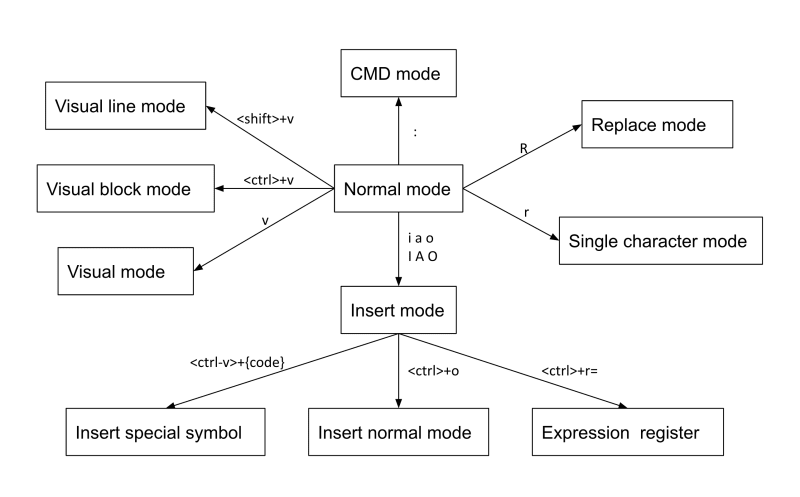
\includegraphics{vimmodes}
  \caption{Simplified Modes in Vim}
  \labfig{vimmodes}
\end{figure}

The figure \reffig{vimmodes} demonstrates how to switch between
the different modes in vim.
\sidenote{
  This is a simplified version of the modes in vim.
  There are other interim modes and other keystrokes
  that toggle the modes. This is shown in detail in
  \reffig{vim-modes}.
}

\begin{figure*}[h]
  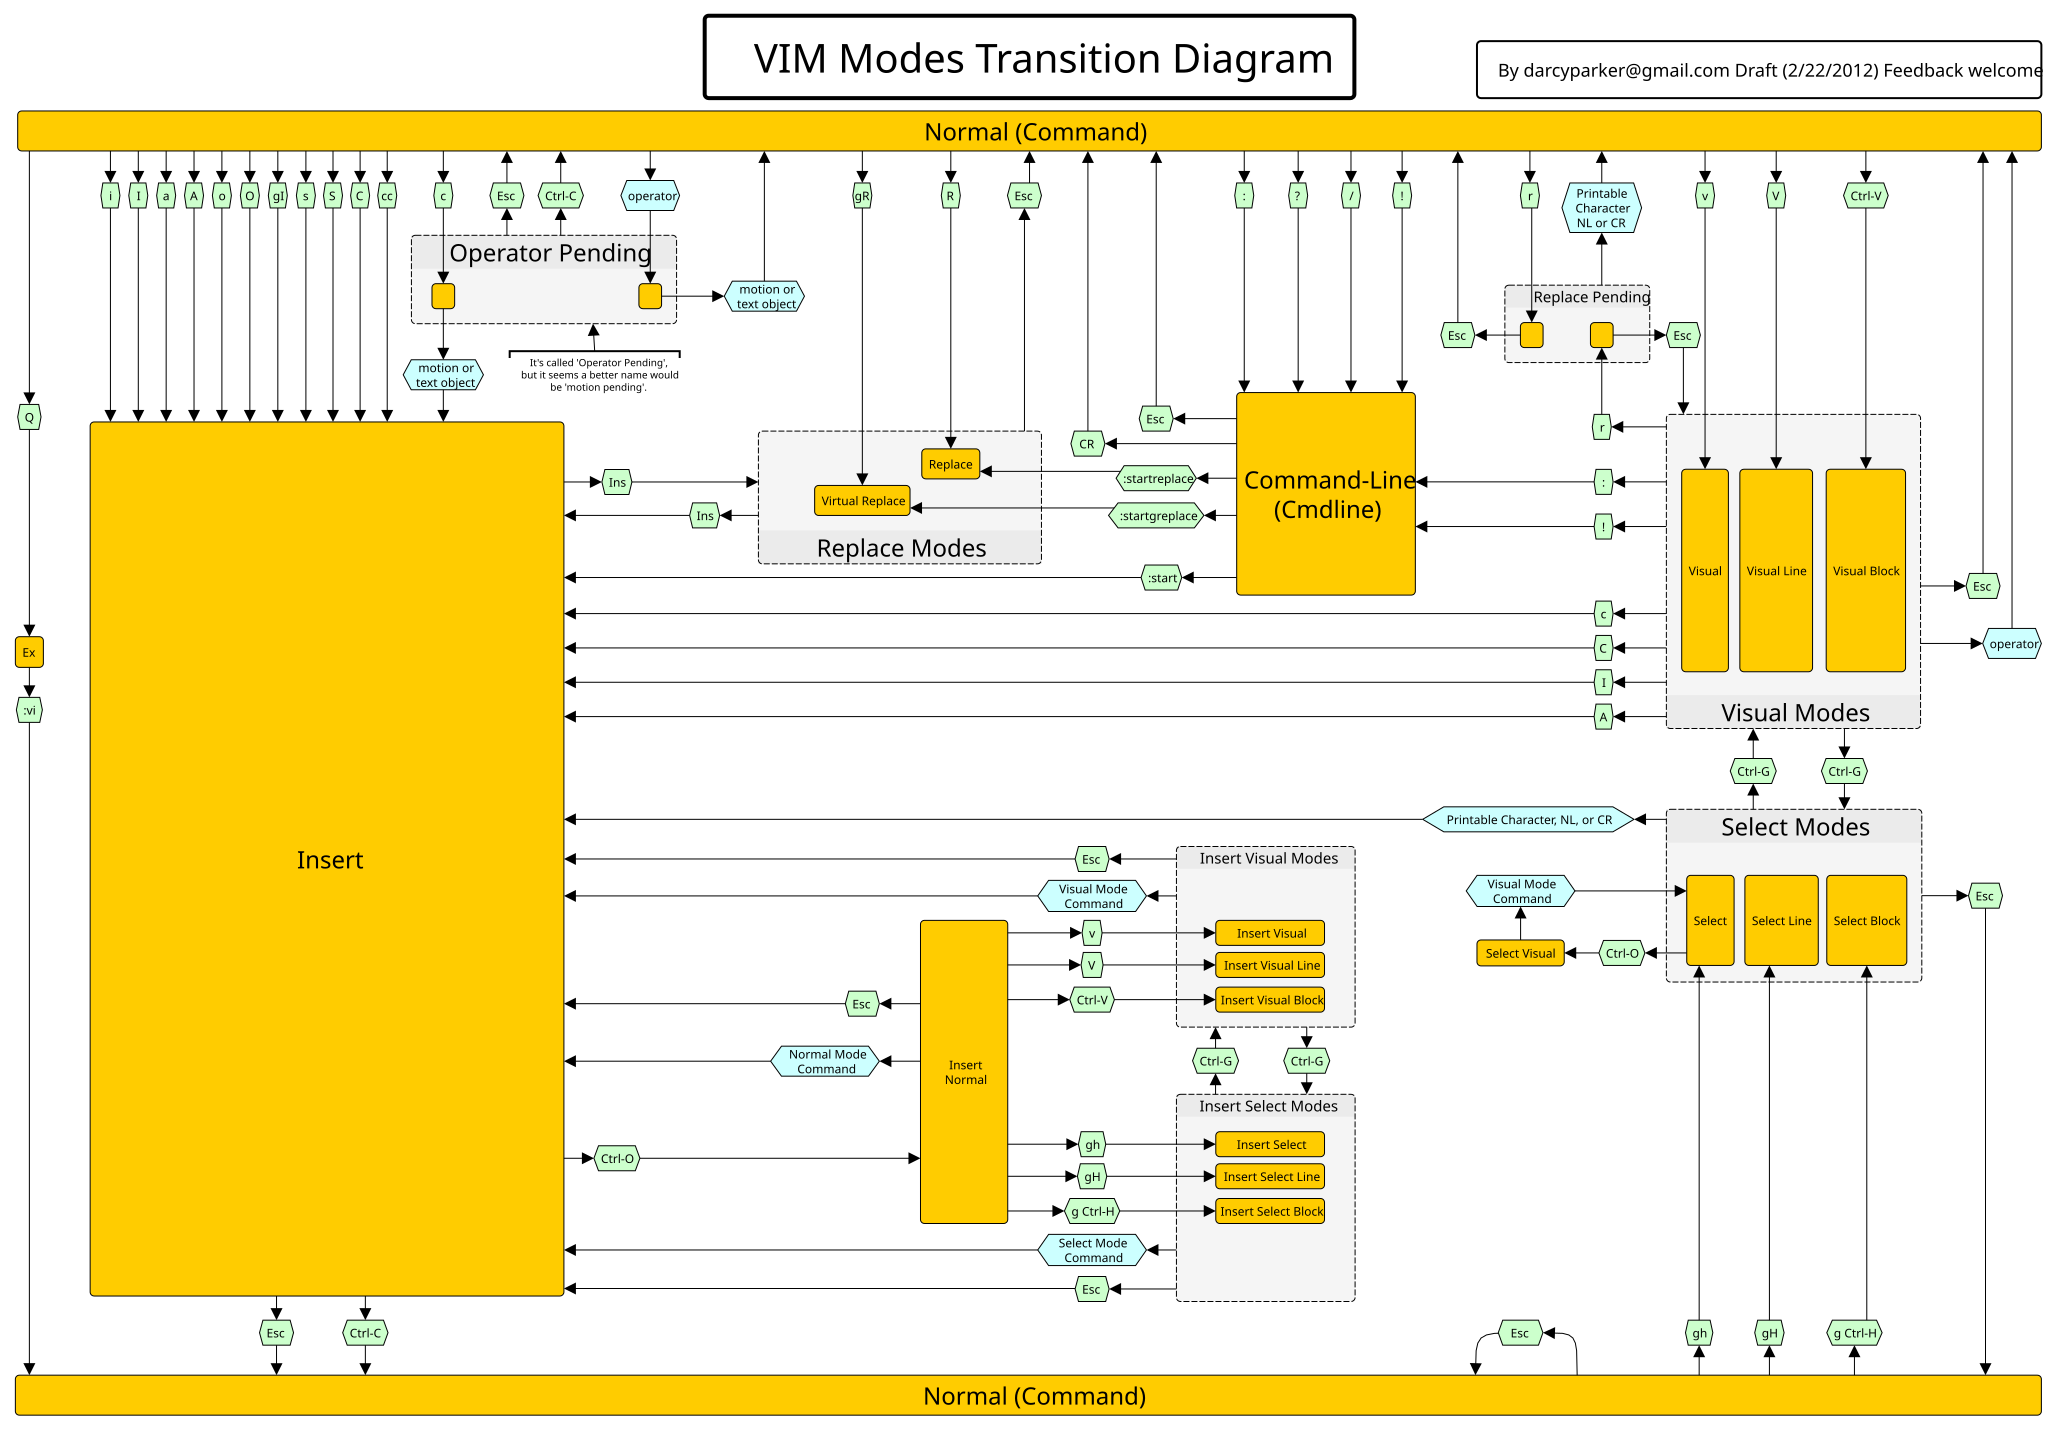
\includegraphics{vim-modes}
  \caption{Detailed Modes in Vim}
  \labfig{vim-modes}
\end{figure*}

\textbf{Commands in Ex mode}

Since we are already familar with commands in
\textbf{ed}, most of the commands are same/similar
in \textbf{ex} mode of vim.

\begin{table}[h!]
  \caption{Ex Commands in Vim}
  \labtab{ex-vim}
  \begin{tabular}{c l}
    \toprule
    Key & Description \\
    \midrule
    \texttt{:f} & show name of file \\
    \texttt{:p} & print current line \\
    \texttt{:a} & append at current line \\
    \texttt{:c} & change current line \\
    \texttt{:d} & delete current line \\
    \texttt{:i} & insert line at current position \\
    \texttt{:j} & join lines \\
    \texttt{:s} & search and replace regex pattern in current line \\
    \texttt{:m} & move current line to position \\
    \texttt{:u} & undo latest change \\
    \texttt{:w [filename]} & write buffer to filename \\
    \texttt{:q} & quit if no change \\
    \texttt{:wq} & write buffer to filename and quit \\
    \texttt{:x} & write buffer to filename and quit \\
    \texttt{:q!} & quit without saving \\
    \texttt{:r filename} & read file contents into buffer \\
    \texttt{:r !command} & read command output into buffer \\
    \texttt{:e filename} & edit a file \\
    \texttt{:sp [filename]} & split the screen and open another file \\
    \texttt{:vsp [filename]} & vertical split the screen and open another file \\
    \bottomrule
  \end{tabular}
\end{table}

There are many more commands in the ex mode of vim.
Along with implementing the original ed commands, it
also has a lot of additional commands to make it more
integrated with the vim editor, such as the ability
to open split windows, new tabs, buffers, and perform
normal mode commands in ex mode.

\textbf{Basic Navigation}

The basic keys for moving around in a text file in vim
are the \texttt{h,j,k,l} keys. They move the cursor
one character to the left, down, up, and right respectively.
These keys are chosen because they are present on the
home row of the keyboard, and do not require the user
to move their hands from the home row to navigate.
\sidenote{
  These were historically chosen because the ADM-3A terminal
  had these keys for navigation as seen in \reffig{adm3a}.
}

Along with these, we have keys to navigate word by word,
or to move to the next pattern match, or the next
paragraph, spelling error, etc.

\begin{table}[h!]
  \caption{Navigation Commands in Vim}
  \labtab{nav-vim}
  \begin{tabular}{c l}
    \toprule
    Key & Description \\
    \midrule
    \texttt{h} & move cursor left \\
    \texttt{j} & move cursor down \\
    \texttt{k} & move cursor up \\
    \texttt{l} & move cursor right \\
    \texttt{w} & move to the beginning of the next word \\
    \texttt{e} & move to the end of the current word \\
    \texttt{b} & move to the beginning of the previous word \\
    \texttt{\%} & move to the matching parenthesis, bracket, or brace \\
    \texttt{0} & move to the beginning of the current line \\
    \texttt{\$} & move to the end of the current line \\
    \texttt{/} & search forward for a pattern \\
    \texttt{?} & search backward for a pattern \\
    \texttt{n} & repeat the last search in the same direction \\
    \texttt{N} & repeat the last search in the opposite direction \\
    \texttt{gg} & move to the first line of the file \\
    \texttt{G} & move to the last line of the file \\
    \texttt{1G} & move to the first line of the file \\
    \texttt{1gg} & move to the first line of the file \\
    \texttt{:1} & move to the first line of the file \\
    \texttt{\{} & move to the beginning of the current paragraph \\
    \texttt{\}} & move to the end of the current paragraph \\
    \texttt{fg} & move cursor to next occurrence of `g' in the line \\
    \texttt{Fg} & move cursor to previous occurrence of `g' in the line \\
    \bottomrule
  \end{tabular}
\end{table}

\textbf{Wait you forgot your cursor behind!}

All of the above commands move the cursor to the
mentioned location. However, if you want to move
the entire screen, and keep the cursor at the
its current position, you can use the \texttt{z}
command along with \texttt{t} to top the line,
\texttt{b} to bottom the line, and \texttt{z} to
center the line.

There are other commands using the \texttt{Ctrl} key
that moves the screen, and not the cursor.

\begin{table}[h!]
  \caption{Moving the Screen Commands in Vim}
  \labtab{screen-vim}
  \begin{tabular}{c l}
    \toprule
    Key & Description \\
    \midrule
    \texttt{Ctrl+F} & move forward one full screen \\
    \texttt{Ctrl+B} & move backward one full screen \\
    \texttt{Ctrl+D} & move forward half a screen \\
    \texttt{Ctrl+U} & move backward half a screen \\
    \texttt{Ctrl+E} & move screen up one line \\
    \texttt{Ctrl+Y} & move screen down one line \\
    \bottomrule
  \end{tabular}
\end{table}

\textbf{Replacing Text}

Usually in other text editors, if you have a word, phrase, or line
which you want to replace with another, you would either press
the backspace or delete key to remove the text, and then type
the new text. However, in vim, there is a more efficient way
to replace text.

\begin{table}[h!]
  \caption{Replacing Text Commands in Vim}
  \labtab{replace-vim}
  \begin{tabular}{c l}
    \toprule
    Key & Description \\
    \midrule
    \texttt{r} & replace the character under the cursor \\
    \texttt{R} & replace the character from the cursor till escape is pressed \\
    \texttt{cw} & change the word under the cursor \\
    \texttt{c4w} & change the next 4 words \\
    \texttt{C} & delete from cursor till end of line and enter insert mode \\
    \texttt{cc} & delete entire line and enter insert mode \\
    \texttt{5cc} & delete next 5 lines and enter insert mode \\
    \texttt{S} & delete entire line and enter insert mode \\
    \texttt{s} & delete character under cursor and enter insert mode \\
    \bottomrule
  \end{tabular}
\end{table}

\textbf{Toggling Case}

You can toggle the case of a character, word, line,
or any arbitrary chunk of the file using the \texttt{~}
or the \texttt{g~} command.

\begin{table}[h!]
  \caption{Toggling Case Commands in Vim}
  \labtab{togglecase-vim}
  \begin{tabular}{c l}
    \toprule
    Key & Description \\
    \midrule
    \texttt{\textasciitilde} & toggle the case of the character under the cursor \\
    \texttt{g~w} & toggle the case of the word under the cursor \\
    \texttt{g~0} & toggle the case from cursor till beginning of line \\
    \texttt{g~\$} & toggle the case from cursor till end of line \\
    \texttt{g~\{} & toggle the case from cursor till previous empty line \\
    \texttt{g~\{} & toggle the case from cursor till next empty line \\
    \texttt{g~\%} & toggle the case from the bracket, brace, or parenthesis till its pair \\
    \bottomrule
  \end{tabular}
\end{table}

You might start to see a pattern emerging here.
Many commands in vim do a particular command,
and on which text it operates is determined by
the character followed by it. Such as \texttt{c}
to change, \texttt{d} to delete, \texttt{y} to yank,
etc. The text on which the command operates is
mentioned using \texttt{w} for the word, \texttt{0}
for till beginning of line, etc.

This is not a coincidence, but rather a design
of vim to make it more efficient to use.
The first command is called the operator command,
and the second command is called the motion command.

Vim follows a \texttt{operator-count-motion} pattern.
For example: \texttt{d2w} deletes the next 2 words.
This makes it very easy to learn and remember commands,
since you are literally typing out what you want to do.

\textbf{Deleting or Cutting Text}

In Vim, the delete command is used to cut text from the file.

\begin{table}[h!]
  \caption{Deleting Text Commands in Vim}
  \labtab{delete-vim}
  \begin{tabular}{c l}
    \toprule
    Key & Description \\
    \midrule
    \texttt{x} & delete the character under the cursor \\
    \texttt{X} & delete the character before the cursor \\
    \texttt{5x} & delete the next 5 characters \\
    \texttt{dw} & delete the word under the cursor \\
    \texttt{d4w} & delete the next 4 words \\
    \texttt{D} & delete from cursor till end of line \\
    \texttt{dd} & delete entire line \\
    \texttt{6dd} & delete next 6 lines \\
    \bottomrule
  \end{tabular}
\end{table}

\textbf{Motion - till, in, around}

By now you should notice that \texttt{dw} doesn't always
delete the word under the cursor. Technically \texttt{dw}
means delete till the beginning of the next word.
So if you press \texttt{dw} at the beginning of a word,
it will delete the word under the cursor. But if your
cursor is in the middle of a word and you type \texttt{dw},
it will only delete the part of the word till the beginning
of the next word from the cursor position.

To delete the entire word under the cursor, regardless of
where the cursor is in the word, you can use the \texttt{diw}
this means \textbf{d}elete \textbf{i}nside \textbf{w}ord.

However, now you may notice that \texttt{diw} doesn't delete
the space after the word. This results in two consequtive spaces,
one from the end of the word, and one from the beginning of the
word being left behind. To delete the space as well, you can use
\texttt{daw} which means \textbf{d}elete \textbf{a}round \textbf{w}ord.

This works not just with \texttt{w} but with any other motion
such as \textbf{d}elete \textbf{i}nside \textbf{p}aragraph,
which will delete the entire paragraph under the cursor,
resulting in two empty lines being left behind,
and \textbf{d}elete \textbf{a}round \textbf{p}aragraph,
which will delete the entire paragraph under the cursor,
and only one empty line being left behind.

Try out the same with deleting inside other items, such as
brackets, parenthesis, braces, quotes, etc. The syntax remains
the same, \texttt{di\{}, \texttt{di[}, \texttt{di(}, \texttt{di"}, \texttt{di'}, etc.

\textbf{Yanking and Pasting Text}

Yes, copying is called yanking in vim. The command to yank
is \texttt{y} and to paste is \texttt{p}.
You can combine \texttt{y} with all the motions and
\textbf{in} and \textbf{around} motions as earlier.
You can also add the count to yank multiple lines or words.

\begin{table}[h!]
  \caption{Deleting Text Commands in Vim}
  \labtab{delete-vim}
  \begin{tabular}{c l}
    \toprule
    Key & Description \\
    \midrule
    \texttt{yy} & yank the entire line \\
    \texttt{yw} & yank the word under the cursor \\
    \vdots & \vdots \\
    \texttt{p} & paste the yanked text after the cursor \\
    \texttt{P} & paste the yanked text before the cursor \\
    \bottomrule
  \end{tabular}
\end{table}

\begin{remark}
  Important to note that the commands
  \begin{lstlisting}
  yy \end{lstlisting}
  and
  \begin{lstlisting}
  0y$ \end{lstlisting}
  are not the same. The first command yanks the entire line,
  including the newline character at the end of the line.
  The second one yanks the entire line, but does not include
  the newline character at the end of the line.
  Thus if you directly press \texttt{p} after the first command,
  it will paste the line below the current line, and if you
  press \texttt{p} after the second command, it will paste
  the line at the end of the current line.
\end{remark}

\textbf{Undo and Redo}

The undo command in vim is \texttt{u} and the redo command
is \texttt{Ctrl+R}. You can undo multiple changes, unlike ed.

\begin{remark}
  If you want to use vim as your primary editor,
  it is highly recommended to install the
  \textbf{mbbill/undotree} plugin. This plugin
  will show you a tree of all the changes you
  have made in the current buffer, and you can
  go to any point in the tree and undo or redo
  changes. This becomes very useful if you undo
  too many changes and by mistake make a new change,
  this changes your branch in undo tree, and you cannot redo
  the changes you undid. With the undotree plugin,
  you can switch branches of the undo tree and redo
  the changes.
\end{remark}

\textbf{Searching and Replacing}

The search command in vim is \texttt{/} for forward search
and \texttt{?} for backward search. You can use the \texttt{n}
command to repeat the last search in the same direction,
and the \texttt{N} command to repeat the last search in the
opposite direction. For example, if you perform forward search
then using the \texttt{n} command will search for the next
occurrence of the pattern in the forward direction, and using
the \texttt{N} command will search for the previous occurrence
of the pattern in the backward direction. However if you perform
a backward search using the \texttt{?} command, then using the
\texttt{n} command will search for the previous occurrence of the
pattern in the backward direction, and using the \texttt{N} command
will search for the next occurrence of the pattern in the forward
direction.

You can also use the \texttt{*} command to search for the word
under the cursor, and the \texttt{\#} command to search for the
previous occurrence of the word under the cursor.

You can perform search and replace using the \texttt{:s} command.
The command takes a line address on which to perform the search
and replace. Usually you can use the \texttt{\%} address to
search in the entire file, or the \texttt{.,\$} address to
search from cursor till the end of the file.

You can also use any line number to specify the address range,
similar to the ed editor.

\begin{lstlisting}
:[addr]s/pattern/replace/[flags]
\end{lstlisting}

The flags at the end of the search and replace command can be
\textbf{g} to replace all occurrences in the line, and
\textbf{c} to confirm each replacement.

The address can be a single line number, a range of line numbers,
or a pattern to search for. The pattern can be a simple string,
or a regular expression.

Some examples of addresses are shown in \reftab{address-vim}.

\begin{table}[h!]
  \caption{Address Types in Search and Replace}
  \labtab{address-vim}
  \begin{tabular}{c l}
    \toprule
    Key & Description \\
    \midrule
    \texttt{m,n} & from line m to line n \\
    \texttt{m} & line m \\
    \texttt{m,\$} & from line m to end of file \\
    \texttt{.,\$} & from current line to end of file \\
    \texttt{1,n} & from line 1 to line n \\
    \texttt{/regex/,n} & from line containing regex to line n \\
    \texttt{m,/regex/} & from line m to line containing regex \\
    \texttt{.,/regex/} & from current line to line containing regex \\
    \texttt{/regex/,.} & from line containing regex to current line \\
    \texttt{1,/regex/} & from the first line to line containing regex \\
    \texttt{/regex/,\$} & from line containing regex to the last line \\
    \texttt{/regex1/;/regex2/} & from line containing regex1 to line containing regex2 \\
    \texttt{\%} & entire file \\
    \bottomrule
  \end{tabular}
\end{table}

\textbf{Insert Mode}

\begin{table}[h!]
  \caption{Keys to enter Insert Mode}
  \labtab{insert-vim}
  \begin{tabular}{c l}
    \toprule
    Key & Description \\
    \midrule
    \texttt{i} & enter insert mode before the cursor \\
    \texttt{a} & enter insert mode after the cursor \\
    \texttt{I} & enter insert mode at the beginning of the line \\
    \texttt{A} & enter insert mode at the end of the line \\
    \texttt{o} & add new line below the current line and enter insert mode \\
    \texttt{O} & add new line above the current line and enter insert mode \\
    \bottomrule
  \end{tabular}
\end{table}

You can enter insert mode from escape mode using the
keys listed in \reftab{insert-vim}.
In insert mode, if you want to insert any non-graphical character,
you can do that by pressing \texttt{Ctrl+V} followed by the
key combination for the character. For example, to insert
a newline character, you can press \texttt{Ctrl+V} followed
by \texttt{Enter}.

These are just the basic commands to get you started with vim.
You can refer to vim cheat sheets present online to get
more familiar with the commands.

\begin{itemize}
  \item \url{https://vim.rtorr.com/} is a good text based HTML cheat sheet for vim.
  \item \url{https://vimcheatsheet.com/} is a paid graphical cheat sheet for vim.
    \sidenote{
      A free version of the graphical cheat sheet is shown in \reffig{vimcheat}.
    }
\end{itemize}

\begin{figure*}[p]
  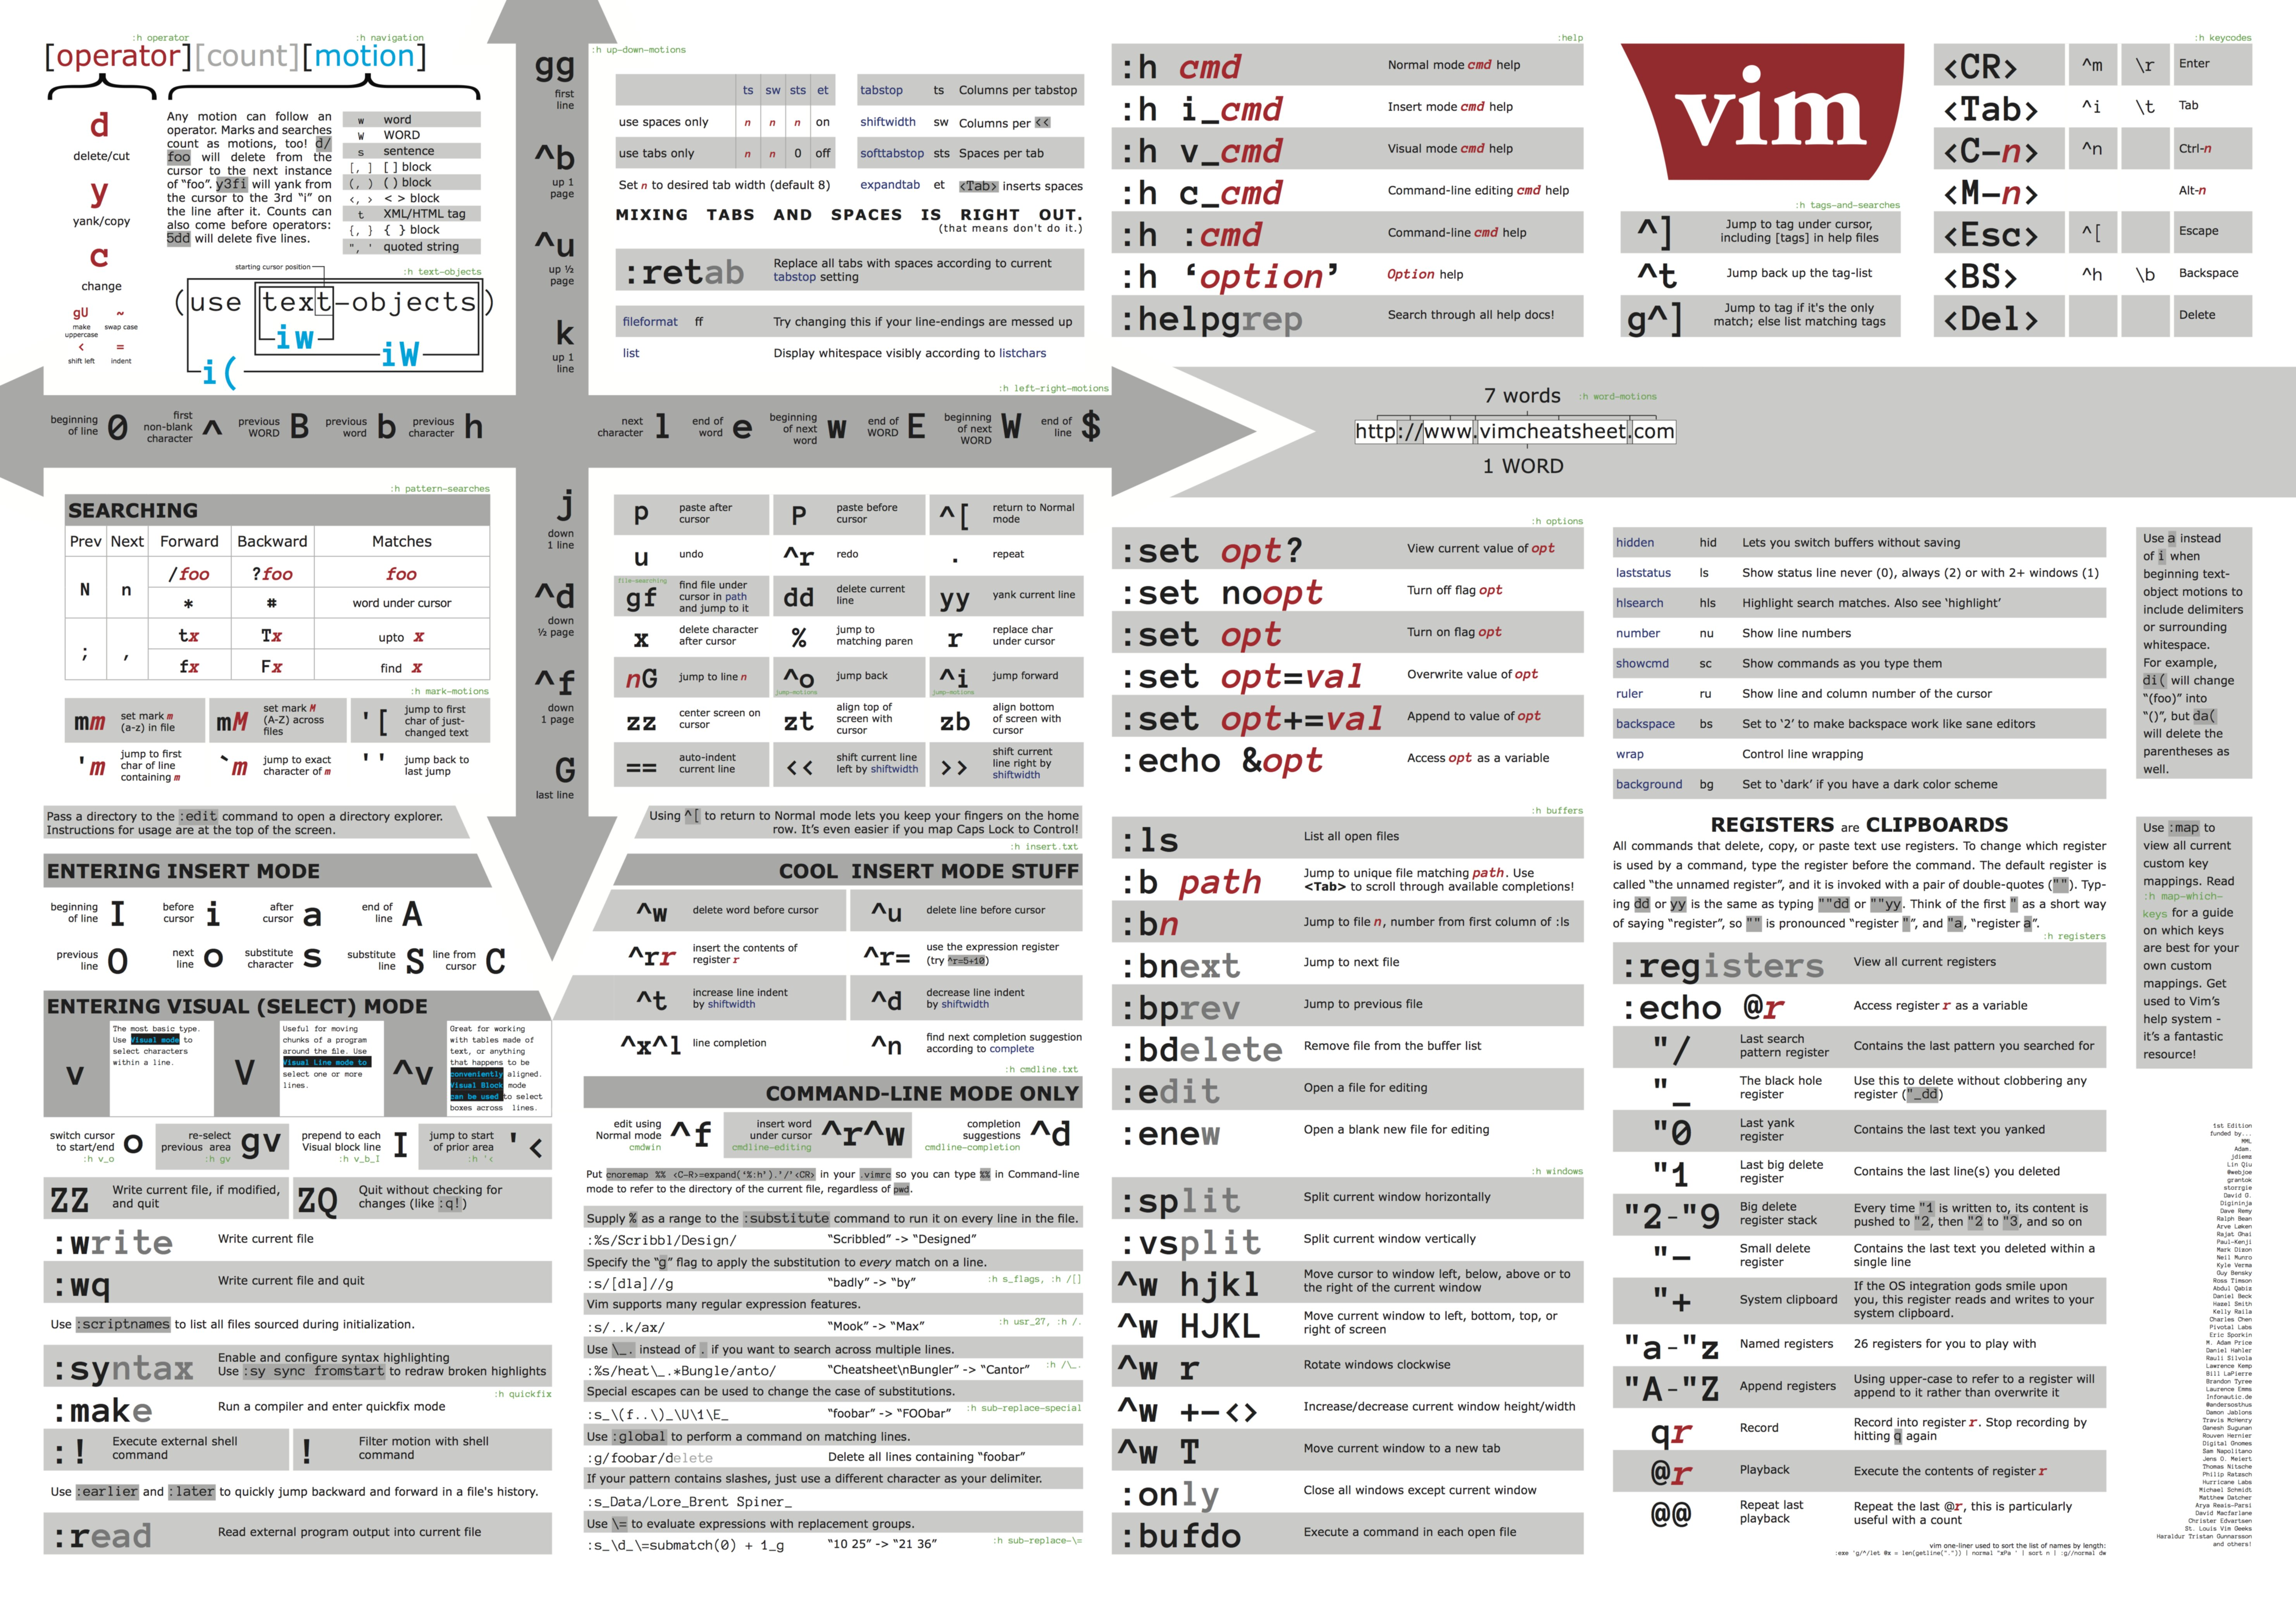
\includegraphics{vimcheat.jpg}
  \caption{Vim Cheat Sheet}
  \labfig{vimcheat}
\end{figure*}

\vfill
\pagebreak
\section{Emacs}

\subsection{History}

Emacs was mostly developed by Richard Stallman and Guy Steele.

\begin{table}[h!]
\caption{History of Emacs}
\labtab{emacshistory}
\centering
\begin{minipage}[t]{.7\linewidth}
\color{gray}
\rule{\linewidth}{1pt}
\ytl{1962}{TECO (Tape Editor and Corrector) was developed at MIT}
\ytl{1976}{Richard Stallman visits Stanford AI Lab and sees Fred Wright's E editor}
\ytl{1978}{Guy Steele accumulates a collection of TECO macros into EMACS}
\ytl{1979}{EMACS becomes MIT's standard text editor}
\ytl{1981}{James Gosling writes Gosling Emacs that runs on UNIX}
\ytl{1984}{Richard Stallman starts GNU Emacs - a free software alternative to Gosling Emacs}
\bigskip
\rule{\linewidth}{1pt}
\end{minipage}
\end{table}

\begin{marginfigure}[-8cm]
  
\includegraphics{emacs}
  \caption{Emacs Logo}
  \labfig{emacs}
\end{marginfigure}


\begin{marginfigure}
  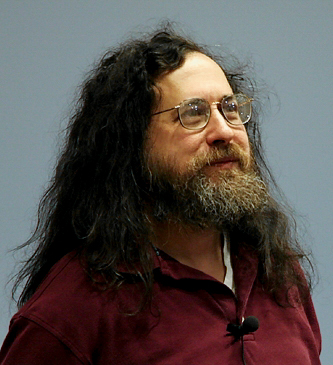
\includegraphics{stallman}
  \caption{Richard Stallman - founder of GNU and FSF projects}
  \labfig{stallman}
\end{marginfigure}

\textbf{TECO}

TECO was developed at MIT in 1962. It was a text editor
used to correct the output of the PDP-1 computer.
It is short for Tape Editor and Corrector.
Unlike most modern text editors,
TECO used separate modes in which the user would either
add text, edit existing text, or display the document
One could not place characters directly into a document
by typing them into TECO, but would instead enter a
character ('i') in the TECO command language telling
it to switch to input mode, enter the required characters,
during which time the edited text was not displayed on
the screen, and finally enter a character (<esc>) to
switch the editor back to command mode. This is very
similar to how vi works.

\textbf{Stallman's Visit to Stanford}

In 1976, Richard Stallman visited the Stanford AI Lab
where he saw Fred Wright's E editor. He was impressed
by E's WYSIWYG
\sidenote{
  What You See Is What You Get
}
interface where you do not need to tackle multiple
modes to edit a text file. This is the default behaviour
of most modern editors now.
He then returned to MIT where he found that
Carl Mikkelsen had added to TECO a combined
display/editing mode called Control-R that allowed
the screen display to be updated each time the user
entered a keystroke. Stallman reimplemented this mode
to run efficiently and added a macro feature to the TECO
display-editing mode that allowed the user to redefine
any keystroke to run a TECO program.

Initially TECO was able to only edit the file
sequentially, page by page. This was due to earlier
memory restrictions of the PDP-1.
Stallman modified TECO to read the entire file into
the buffer, and then edit the buffer in memory
allowing for random access to the file.

\textbf{Too Many Macros!}

The new version of TECO quickly became popular at
the AI Lab and soon accumulated a large collection
of custom macros whose names often ended in MAC or
MACS, which stood for macro.
This quickly got out of hand as there were many
divergent macros, and a user would be totally
lost when using a co-worker's terminal.

\begin{marginfigure}
  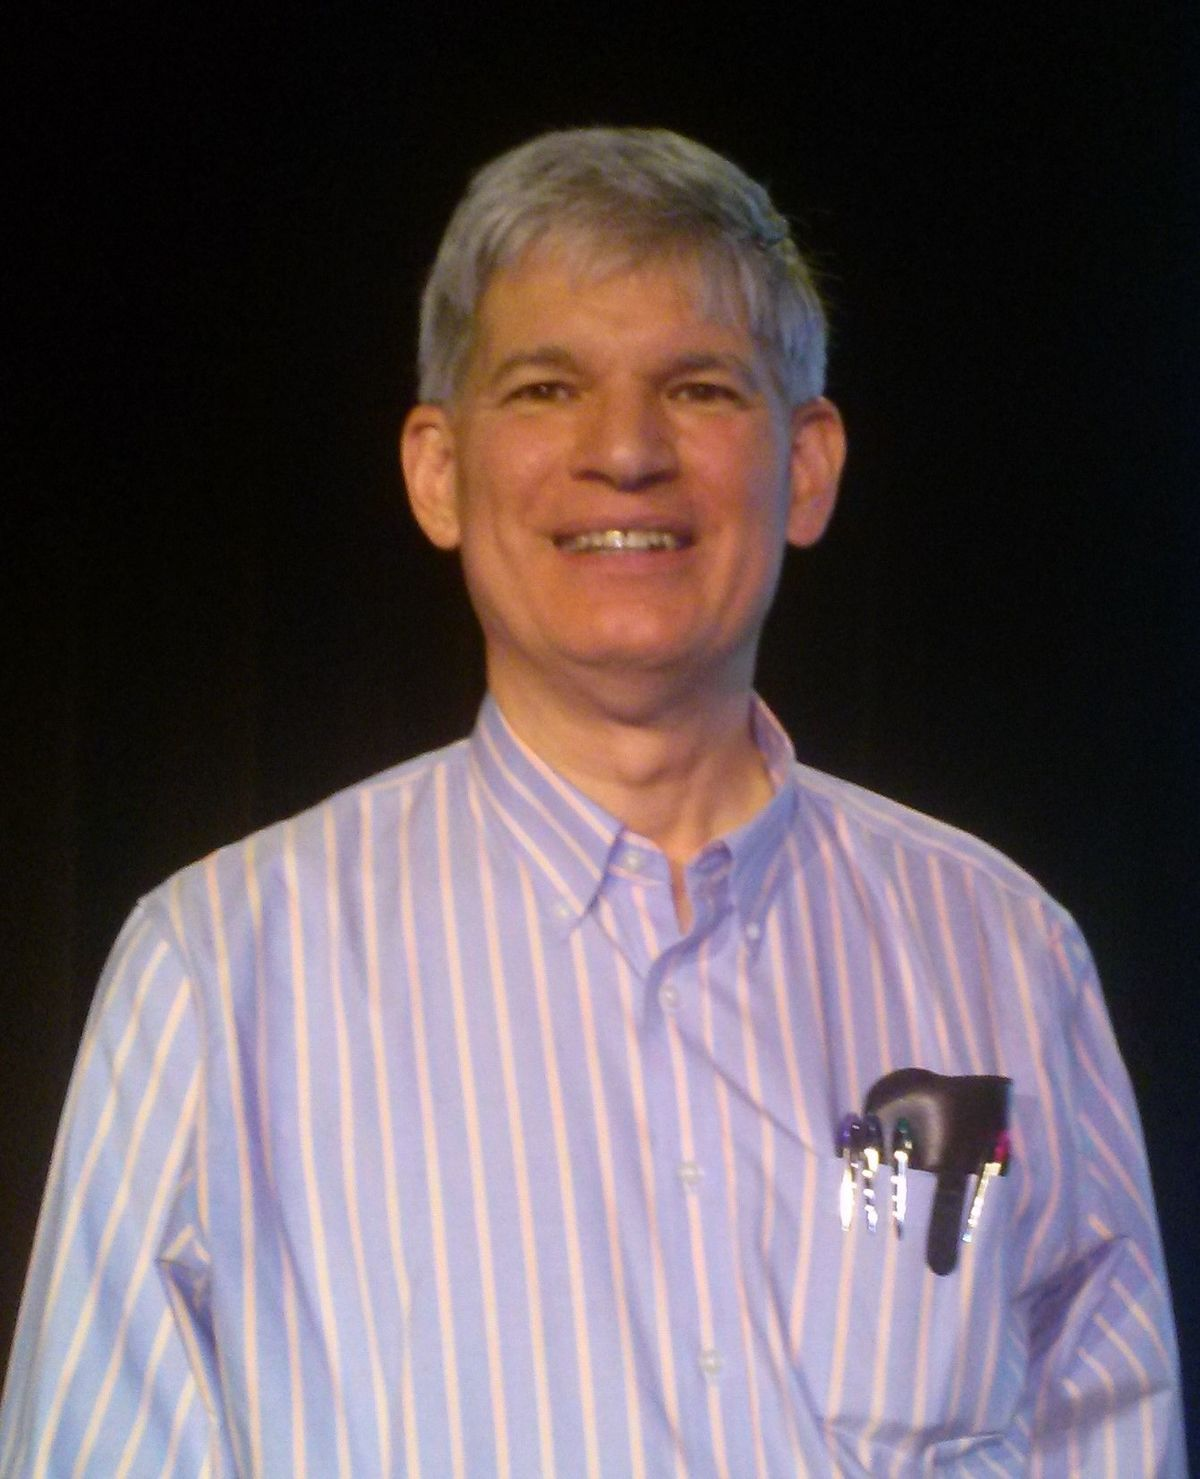
\includegraphics{steele}
  \caption{Guy L. Steele Jr. combined many divergent TECO with macros to create EMACS}
  \labfig{steele}
\end{marginfigure}


In 1979, Guy Steele combined many of the popular
macros into a single file, which he called EMACS,
which stood for Editing MACroS, or E with MACroS.

To prevent thousands of forks of EMACS, Stallman
declared that
`EMACS was distributed on a basis of communal sharing,
which means all improvements must be given back to me
to be incorporated and distributed.'

Till now, the EMACS, like TECO, ran on the PDP-10
which ran the ITS operating system and not UNIX.

\textbf{EINE ZWEI SINE and other clones}

No, that is not German.
These are some of the popular clones of EMACS
made for other operating systems.

EINE
\sidenote{
  EINE stands for Eine Is Not EMACS
}
was a text editor developed in the late 1970s.
In terms of features, its goal was to `do what Stallman's
PDP-10 (original) Emacs does'.
Unlike the original TECO-based Emacs, but like Multics Emacs,
EINE was written in Lisp. It used Lisp Machine Lisp.

In the 1980s, EINE was developed into ZWEI
\sidenote{
  ZWEI stands for ZWEI Was Eine Initially
}.
Innovations included programmability in Lisp Machine Lisp,
and a new and more flexible doubly linked
list method of internally representing buffers.

\marginnote{
  These kinds of recursive acronyms are common in the
  \*nix world. For example, GNU stands for GNU's Not Unix,
  WINE (A compatibility layer to run Windows applications)
  is short for WINE Is Not an Emulator.
}

SINE
\sidenote{
  SINE stands for SINE Is Not EINE
}
was written by Owen Theodore Anderson in 1981.

In 1978, Bernard Greenberg wrote a version of EMACS
for the Multics operating system called Multics EMACS.
This used Multics Lisp.


\begin{marginfigure}
  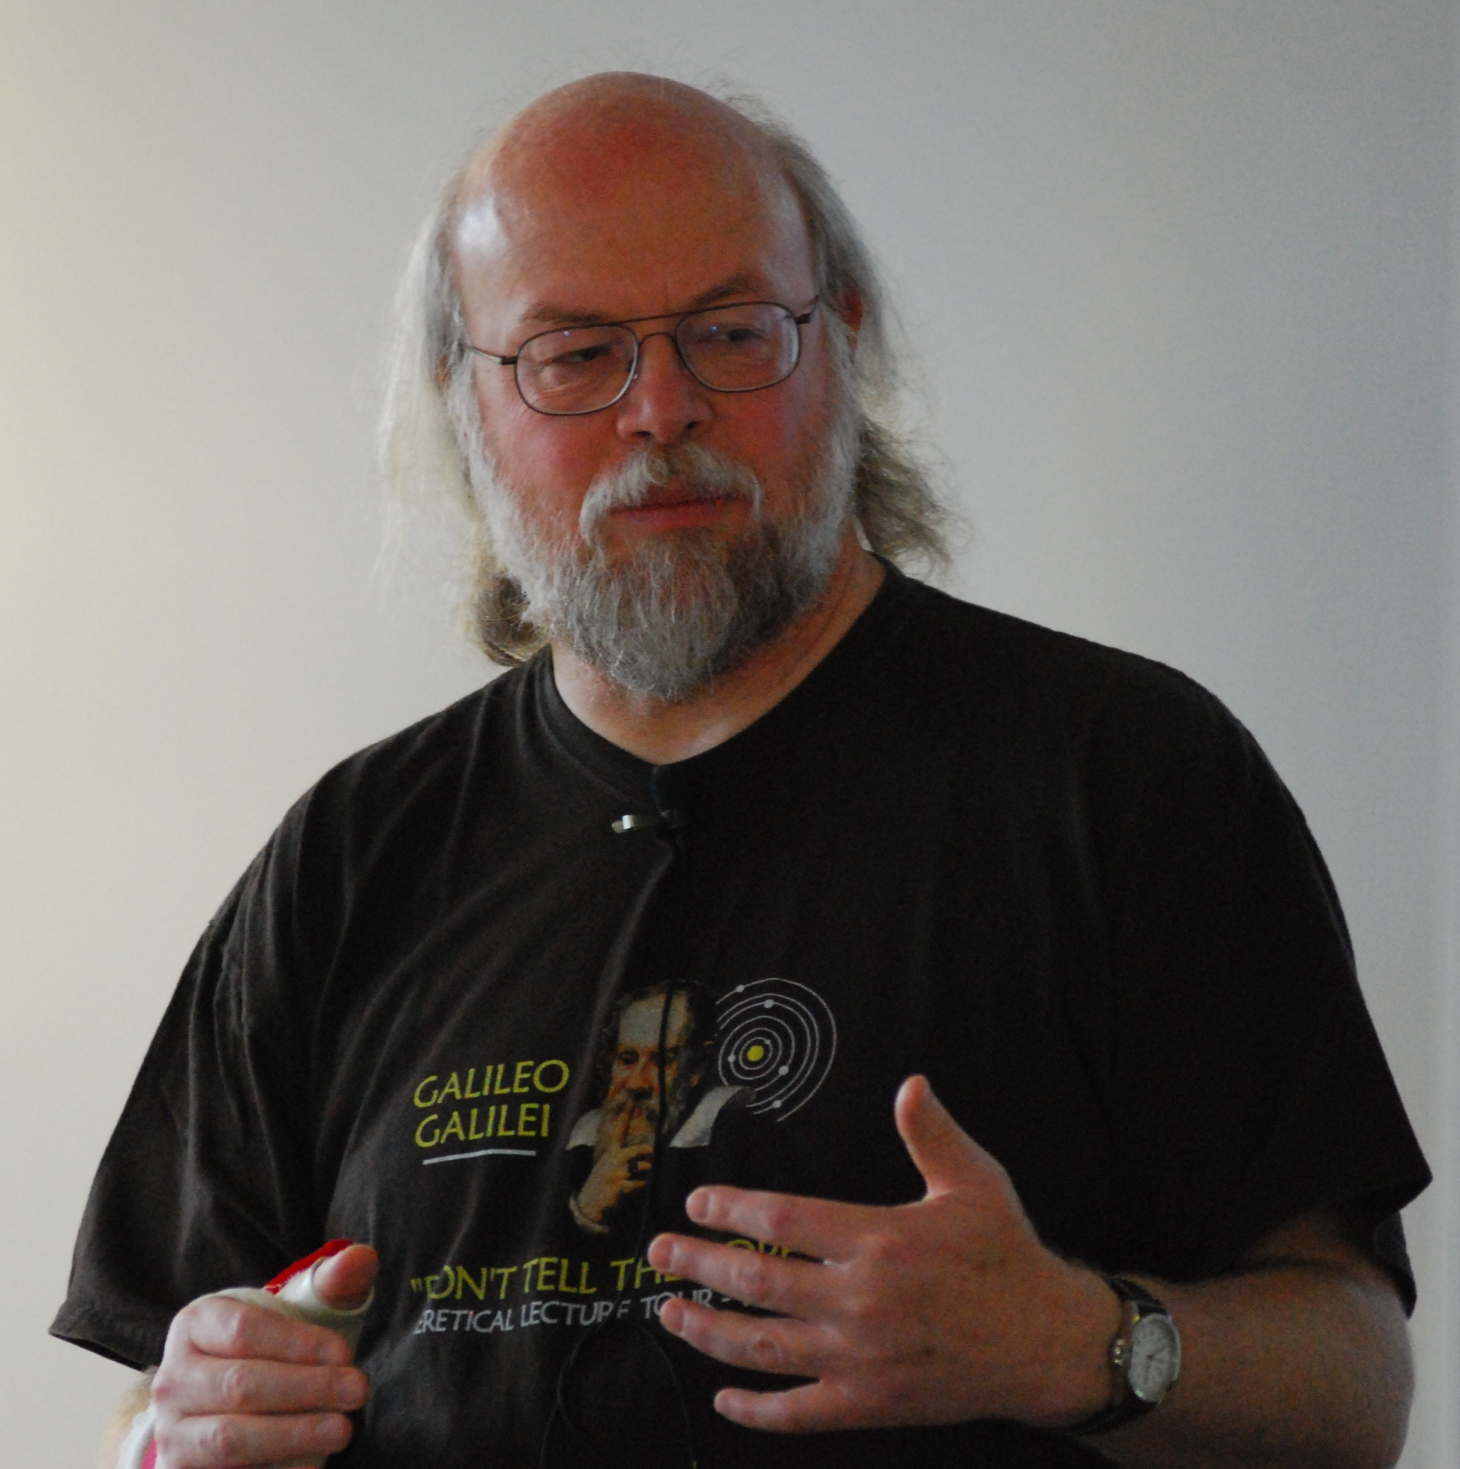
\includegraphics{gosling}
  \caption{James Gosling - creator of Gosling Emacs and later Java}
  \labfig{gosling}
\end{marginfigure}

\textbf{Gosling Emacs}

In 1981, James Gosling wrote Gosling Emacs for UNIX.
It was written in C and used Mocklisp, a language with
lisp-like syntax, but not a lisp. It was not free software.

\textbf{GNU Emacs}

In 1983, Stallman started the GNU project to create a
free software alternatives to proprietary softwares
and ultimately to create a free
\sidenote{
Recall from the previous chapter that free software
does not mean a software provided gratis, but a software
which respects the user's freedom to run, copy, distribute,
and modify the software. It is like free speech, not free beer.
}
operating system.

In 1984, Stallman started GNU Emacs, a free software
alternative to Gosling Emacs. It was written in C and
used a true Lisp dialect, Emacs Lisp as the extension
language. Emacs Lisp was also implemented in C.
This is the version of Emacs that is most popular today
and available on most operating systems repositories.

\textbf{How the developer's keyboard influences the editors they make}

Remember that ed was made while using \textbf{ADM-3A}
which looked like \reffig{adm3a-real}.

\begin{marginfigure}
  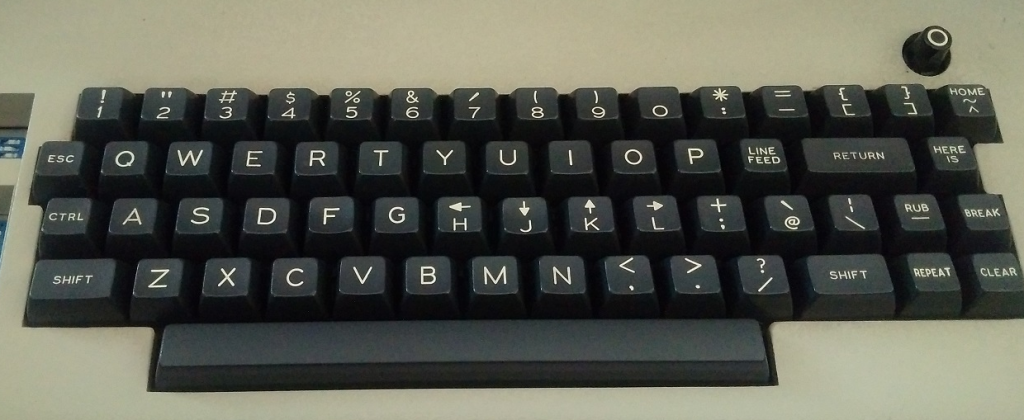
\includegraphics{adm3a-real}
  \caption{ADM-3A terminal}
  \labfig{adm3a-real}
\end{marginfigure}

Whereas emacs was made while the \textbf{Knight keyboard}
and the \textbf{Space Cadet keyboard} were in use, which
can be seen in \reffig{space-cadet}.

\begin{marginfigure}
  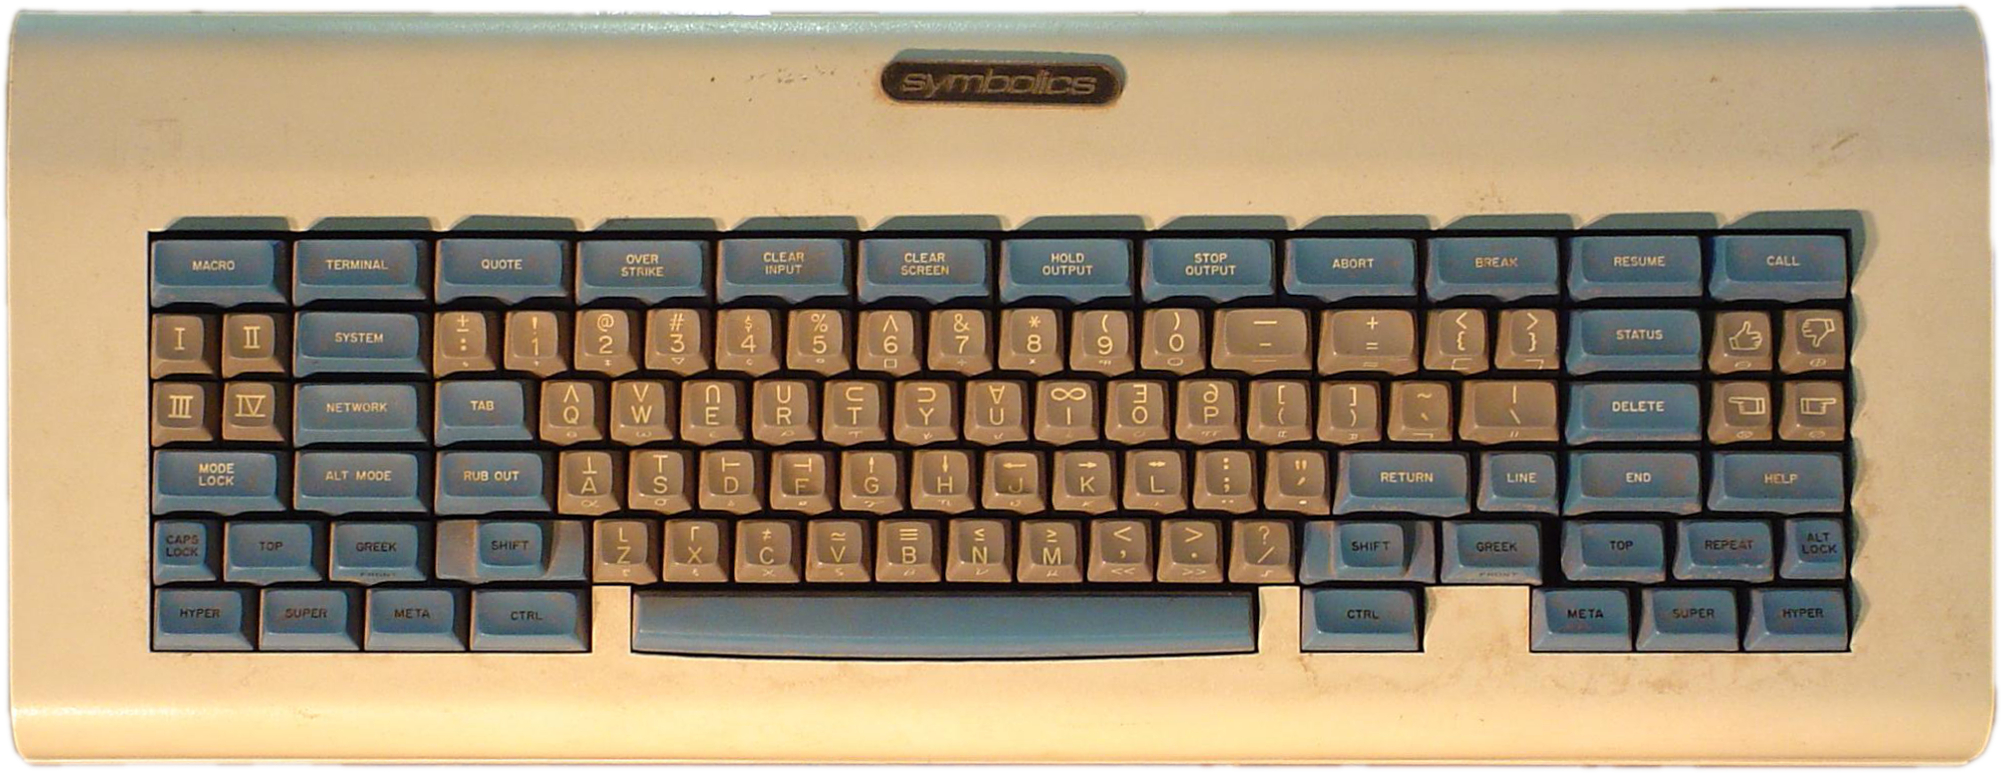
\includegraphics{space-cadet}
  \caption{Space Cadet Keyboard}
  \labfig{space-cadet}
\end{marginfigure}

Notice how the ADM-3A has very limited modifier keys, and
does not even have arrow keys. Instead it uses \texttt{h,j,k,l}
keys as arrow keys with a modifier. This is why vi uses
mostly key combinations and a modal interface.
Vi also uses the \texttt{Esc} key to switch between modes,
which is present conveniently in place of the Caps Lock or Tab key
in modern keyboard layouts.

The Space Cadet keyboard has many modifier keys, and even
a key for the Meta key. This is why emacs uses many key
modifier combinations, and has a lot of keybindings.

\subsection{Exploring Emacs}

This is not a complete overview of Emacs, or even its
keybindings. A more detailed reference card can be
found on their
\href{https://www.gnu.org/software/emacs/refcards/pdf/refcard.pdf}{website}.

\textbf{Opening a File}

We can open a file in emacs by providing its
filename as an argument to the emacs executable.

\begin{lstlisting}[language=bash]
$ emacs test.txt
\end{lstlisting}

Most of emacs keybindings use modifier keys such as
the \texttt{Ctrl} key, and the \texttt{Meta} key.
The \texttt{Meta} key is usually the \texttt{Alt} key
in modern keyboards. In the reference manual and here,
we will be representing the \texttt{Meta} key as \texttt{M-}
and the \texttt{Ctrl} key as \texttt{C-}.

\textbf{Basic Navigation}

These keys are used to move around in the file.
Like vim, emacs also focusses on keeping the hands
free from the mouse, and on the keyboard.
All the navigation can be done through the keyboard.

\begin{table}[h!]
  \caption{Navigation Commands in Emacs}
  \labtab{nav-emacs}
  \begin{tabular}{c l}
    \toprule
    Key & Description \\
    \midrule
    \texttt{C-p} & move up one line \\
    \texttt{C-b} & move left one char \\
    \texttt{C-f} & move right one char \\
    \texttt{C-n} & move down one line \\
    \texttt{C-a} & goto beginning of current line \\
    \texttt{C-e} & goto end of current line \\
    \texttt{C-v} & move forward one screen \\
    \texttt{M-<} & move to first line of the file \\
    \texttt{M-b} & move left to previous word \\
    \texttt{M-f} & move right to next word \\
    \texttt{M->} & move to last line of the file \\
    \texttt{M-a} & move to beginning of current sentence \\
    \texttt{M-e} & move to end of current sentence \\
    \texttt{M-v} & move back one screen \\
    \bottomrule
  \end{tabular}
\end{table}

\textbf{Exiting Emacs}

We can exit emacs either with or without saving the file.
We can also suspend emacs and return to the shell.
This is a keymapping of the shell, and not of emacs.

\begin{table}[h!]
  \caption{Exiting Emacs Commands}
  \labtab{exit-emacs}
  \begin{tabular}{c l}
    \toprule
    Key & Description \\
    \midrule
    \texttt{C-x C-s} & save buffer to file \\
    \texttt{C-z} & suspend emacs \\
    \texttt{C-x C-c} & exit emacs and stop it \\
    \bottomrule
  \end{tabular}
\end{table}

\textbf{Searching Text}

Emacs can search for a fixed string, or a regular expression
and replace it with another string.

\begin{table}[h!]
  \caption{Searching Text Commands in Emacs}
  \labtab{search-emacs}
  \begin{tabular}{c l}
    \toprule
    Key & Description \\
    \midrule
    \texttt{C-s} & search forward \\
    \texttt{C-r} & search backward \\
    \texttt{M-x} & replace string \\
    \bottomrule
  \end{tabular}
\end{table}

\textbf{Copying and Pasting}

Copying can done by marking the region, and then copying it.

\begin{table}[h!]
  \caption{Copying and Pasting Commands in Emacs}
  \labtab{copy-emacs}
  \begin{tabular}{c l}
    \toprule
    Key & Description \\
    \midrule
    \texttt{M-backspace} & cut the word before cursor \\
    \texttt{M-d} & cut the word after cursor \\
    \texttt{M-w} & copy the region \\
    \texttt{C-w} & cut the region \\
    \texttt{C-y} & paste the region \\
    \texttt{C-k} & cut from cursor to end of line \\
    \texttt{M-k} & cut from cursor to end of sentence \\
    \bottomrule
  \end{tabular}
\end{table}

\vfill
\pagebreak
\section{Nano}

\begin{marginfigure}
  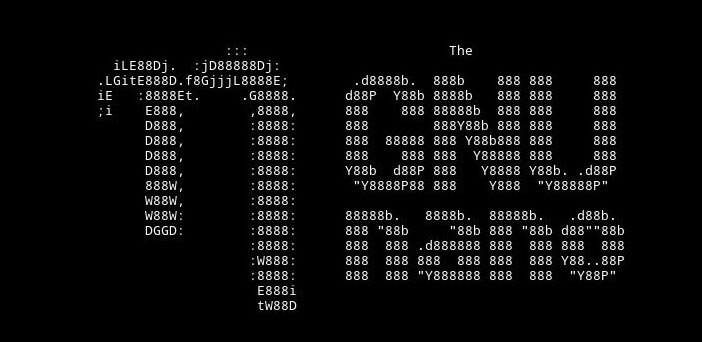
\includegraphics{nano}
  \caption{Nano Text Editor}
  \labfig{nano}
\end{marginfigure}

Although vim and emacs are the most popular
command line text editors, nano is also a very
useful text editor for beginners. It is very
simple and does not have a steep learning curve.

It is a non-modal text editor, which means that
it does not have different modes for different
actions. You can directly start typing text
as soon as you open \textbf{nano}.

Although it uses modifier keys to invoke commands,
it does not have a lot of commands as vim or emacs.

\subsection{History}

Pine
\sidenote{
  It is believed that pine stands for
  Pine is Not Elm, Elm being another
  text-based email client.
  However, the author clarifies that
  it was not named with that in mind.
  Although if a backronym was to be made,
  he prefered `Pine is Nearly Elm' or
  `Pine is No-longer Elm'
}
was a text-based email client developed at the
University of Washington. It was created in 1989.
The email client also had a text editor built in
called Pico.

Although the license of Pine and Pico may seem
open source, it was not. The license was restrictive
and did not allow for modification or redistribution.
\sidenote{
Up to version 3.91, the Pine license was similar to BSD, and it stated that
`Permission to use, copy, modify, and distribute this software and its documentation for any purpose and without fee to the University of Washington is hereby granted ...'
The university registered a trademark for the Pine name with respect to `computer programs used in communication and electronic mail applications' in March 1995.
From version 3.92, the holder of the copyright, the University of Washington, changed the license so that even if the source code was still available, they did not allow modifications and changes to Pine to be distributed by anyone other than themselves. They also claimed that even the old license never allowed distribution of modified versions.
}

Due to this, many people created clones of Pico
with free software licenses. One of the most popular
clones was TIP (TIP isn't Pico) which was created by
Chris Allegretta in 1999. Later in 2000 the name was
changed to Nano.
\sidenote{
  Mathematically, nano is $10^{-9}$ or one billionth.
  and pico is $10^{-12}$ or one trillionth.
  or put relatively, nano is 1000 times bigger than pico,
  although the size of nano binary is smaller than pico.
}
In 2001, nano became part of the GNU project.

GNU nano implements several features that Pico lacks,
including syntax highlighting, line numbers,
regular expression search and replace,
line-by-line scrolling, multiple buffers,
indenting groups of lines, rebindable key support,
and the undoing and redoing of edit changes.

In most modern linux systems, the \textbf{nano}
binary is present along with the \textbf{pico}
binary, which is actually a symbolic link to the
\textbf{nano} binary.

You can explore this by finding the path of the
executable using the \texttt{which} command
and long-listing the executable.

\begin{lstlisting}[language=bash]
$ which pico
/usr/bin/pico
$ ls -l /usr/bin/pico
lrwxrwxrwx 1 root root 22 Sep  6  2023 /usr/bin/pico -> /etc/alternatives/pico
$ ls -l /etc/alternatives/pico
lrwxrwxrwx 1 root root 9 Sep  6  2023 /etc/alternatives/pico -> /bin/nano
\end{lstlisting}

\begin{remark}
  Note that here we have a symlink to another symlink.
  Theoretically, you can extend to as many levels of
  chained symlinks as you want.
  Thus, to find the final sink of the symlink chain,
  you can use the \texttt{readlink -f} command or
  the \texttt{realpath} command.
\end{remark}

\begin{lstlisting}[language=bash]
$ realpath $(which pico)
/usr/bin/nano
\end{lstlisting}

\subsection{Exploring Nano}

In nano, the Control key is represented by the \textasciicircum symbol.
The Meta or Alt key is represented by the \texttt{M-}.

\textbf{File Handling}

You can open a file in nano by providing the filename
as an argument to the nano executable.

\begin{lstlisting}[language=bash]
$ nano test.txt
\end{lstlisting}

\begin{table}[h!]
  \caption{File Handling Commands in Nano}
  \labtab{file-nano}
  \begin{tabular}{c l}
    \toprule
    Key & Description \\
    \midrule
    \texttt{\textasciicircum S} & save the file \\
    \texttt{\textasciicircum O} & save the file with a new name \\
    \texttt{\textasciicircum X} & exit nano \\
    \bottomrule
  \end{tabular}
\end{table}

\textbf{Editing}

Nano is a simple editor, and you can do without learning
any more commands than the ones listed above, but here
are some more basic commands for editing text.

\begin{table}[h!]
  \caption{Editing Commands in Nano}
  \labtab{edit-nano}
  \begin{tabular}{c l}
    \toprule
    Key & Description \\
    \midrule
    \texttt{\textasciicircum K} & cut current line and save in cutbuffer \\
    \texttt{M-6} & copy current line and save in cutbuffer \\
    \texttt{\textasciicircum U} & paste contents of cutbuffer \\
    \texttt{M-T} & cut until end of buffer \\
    \texttt{\textasciicircum ]} & complete current word \\
    \texttt{M-U} & undo last action \\
    \texttt{M-E} & redo last undone action \\
    \texttt{\textasciicircum J} & justify the current paragraph \\
    \texttt{M-J} & justify the entire file \\
    \texttt{M-:} & start/stop recording a macro \\
    \texttt{M-;} & run the last recorded macro \\
    \texttt{F12} & invoke the spell checker, if available \\
    \bottomrule
  \end{tabular}
\end{table}

There are many more commands in nano, but they are
omitted from here for brevity. You can find the
complete list of keybindings by pressing \texttt{\textasciicircum G}
key in nano, or by running \lstinline[language=bash]{info nano}.
\marginnote{
  You can also find third-party cheat sheets
  \href{https://www.cheatsheet.wtf/Nano/}{online}.
}

\subsection{Editing A Script in Nano}

Since learning nano is mostly to be able to edit
a text file even if you are not familiar with
either vim or emacs, let us try to edit a simple
script file to confirm that you can use nano.

\begin{lstlisting}[language=bash]
$ touch myscript.sh
$ chmod u+x myscript.sh
$ nano myscript.sh
\end{lstlisting}

Now try to write a simple script in the file.
An example script is shown below.

\begin{lstlisting}[language=bash]
#!/bin/bash
read -rp 'What is your name? ' name
echo "Hello $name"
date=$(date "+%H:%M on a %A")
echo "Currently it is $date"
\end{lstlisting}

\marginnote{
  If you do not understand how the script works,
  do not worry. It will be covered in depth in
  later chapters.
}

Now save the file by pressing \texttt{\textasciicircum S}
\begin{remark}
  In some systems, the \texttt{\textasciicircum S} key
  will freeze the terminal. Any key you press after this
  will seem to not have any effect.
  This is because it is interpreted as the \texttt{XOFF}
  and is used to lock the scrolling of the terminal.
  To unfreeze the terminal, press \texttt{\textasciicircum Q}.
  In such a system, you can save the file by pressing
  \texttt{\textasciicircum O} and then typing out the
  name of the file if not present already, and pressing
  Enter.
  To disable this behaviour, you can add the line
  \begin{lstlisting}[language=bash]
  set -ixon \end{lstlisting}
  to your \texttt{.bashrc} file.
\end{remark}
and exit nano by pressing \texttt{\textasciicircum X}.

Now you can run the script by typing

\begin{lstlisting}[language=bash]
$ ./myscript.sh
What is your name? Sayan
Hello Sayan
Currently it is 21:50 on a Tuesday
\end{lstlisting}

Now that we are able to edit a text file using text editors,
we are ready to write scripts to solve problems.
